\documentclass[review]{elsarticle}

\usepackage{lineno,hyperref}

\modulolinenumbers[5]

\journal{Journal of \LaTeX\ Templates}

%%%%%%%%%%%%%%%%%%%%%%%
%% Elsevier bibliography styles
%%%%%%%%%%%%%%%%%%%%%%%
%% To change the style, put a % in front of the second line of the current style and
%% remove the % from the second line of the style you would like to use.
%%%%%%%%%%%%%%%%%%%%%%%

%% Numbered
%\bibliographystyle{model1-num-names}

%% Numbered without titles
%\bibliographystyle{model1a-num-names}

%% Harvard
\bibliographystyle{model2-names.bst}\biboptions{authoryear}

%% Vancouver numbered
%\usepackage{numcompress}\bibliographystyle{model3-num-names}

%% Vancouver name/year
%\usepackage{numcompress}\bibliographystyle{model4-names}\biboptions{authoryear}

%% APA style
%\bibliographystyle{model5-names}\biboptions{authoryear}

%% AMA style
%\usepackage{numcompress}\bibliographystyle{model6-num-names}

%% `Elsevier LaTeX' style
%\bibliographystyle{elsarticle-num}
%%%%%%%%%%%%%%%%%%%%%%%
\usepackage{bm}
\usepackage{amsmath}
\usepackage{amssymb}
\usepackage{amsthm}
\usepackage{graphicx}
\usepackage{color}
\usepackage{booktabs}
\usepackage[linesnumbered,ruled]{algorithm2e}


\DeclareMathOperator{\mytr}{tr}
\DeclareMathOperator{\mydiag}{diag}
\DeclareMathOperator{\myrank}{Rank}
\DeclareMathOperator{\myE}{E}
\DeclareMathOperator{\myVar}{Var}

\newcommand{\BP}{\mathbf{P}}

\theoremstyle{plain}
\newtheorem{theorem}{\quad\quad Theorem}
\newtheorem{proposition}{\quad\quad Proposition}
\newtheorem{corollary}{\quad\quad Corollary}
\newtheorem{lemma}{Lemma}
\newtheorem{example}{Example}
\newtheorem{assumption}{\quad\quad Assumption}
\newtheorem{condition}{Condition}

\theoremstyle{definition}
\newtheorem{remark}{\quad\quad Remark}
\theoremstyle{remark}




\begin{document}

\begin{frontmatter}

\title{A feasible high dimensional randomization test for mean vector}
%\tnotetext[mytitlenote]{Fully documented templates are available in the elsarticle package on \href{http://www.ctan.org/tex-archive/macros/latex/contrib/elsarticle}{CTAN}.}

    \author[mymainaddress]{Rui Wang}
    \author[mymainaddress,mysecondaryaddress]{Xingzhong Xu\corref{mycorrespondingauthor}}
\cortext[mycorrespondingauthor]{Corresponding author}
\ead{xuxz@bit.edu.cn}
    \address[mymainaddress]{School of Mathematics and Statistics, Beijing Institute of Technology, Beijing 
    100081,China}
    \address[mysecondaryaddress]{Beijing Key Laboratory on MCAACI, Beijing Institute of Technology, Beijing 100081,China}
    
    
\begin{abstract}
    The strength of randomization tests is that the size of the test is exact under certain symmetry assumption for distribution.
    In this paper, we study a randomization test for mean vector in high dimensional setting. 
    In classical statistics, a major down-side to randomization tests is that they are computational intensive.    
    Surprisingly, it is not the case in high dimensional setting.
    We give an implementation of the randomization procedure, the time complexity of which does not rely on data dimension. 
    The theoretical property of randomization test is another important issue.
    So far, the asymptotic behaviors of randomization tests have only been studied in fixed dimension case.
    We investigate the asymptotic behavior of the randomization test in high dimensional setting.
    It turns out that even if the symmetry assumption is violated, the randomization test has correct level asymptotically.
    The asymptotic power function is also given.
    With fast implementation and good theoretical properties, the randomization test can be recommended in practice.
\end{abstract}

\begin{keyword}
    Asymptotic power function \sep High dimension \sep Randomization test\sep Symmetry assumption 
%\MSC[2010] 00-01\sep  99-00
\end{keyword}

\end{frontmatter}

%\linenumbers


\section{Introduction}

Let $X_{1},\ldots,X_{n}$ be independent and identically distributed (iid) $p$-dimensional random vectors with mean vector $\mu={(\mu_1,\ldots,\mu_p)}^T$ and covariance matrix $\Sigma$. In this paper, we consider the randomization test procedure for testing the hypotheses
\begin{equation}\label{ourHy}
    H_0:\mu=0_p\quad \textrm{versus} \quad H_1:\mu\neq 0_p.
\end{equation}


%Tests for hypotheses~\eqref{ourHy} has been extensively studied by many researchers.
A classical test statistic for hypotheses~\eqref{ourHy} is Hotelling's $T^2$, defined as
    $
    n\bar{X}^T S^{-1}\bar{X}
    $,
where $\bar{X}=n^{-1}\sum_{i=1}^n X_i$ and $S=(n-1)^{-1}\sum_{i=1}^n (X_i-\bar{X}) (X_i-\bar{X})^T$ are the sample mean vector and sample covariance matrix, respectively.
Under normal distribution, Hotelling's $T^2$ is the likelihood ratio test and enjoys desirable properties in fixed $p$ case. See, for example,~\cite{andersonMultivariate}.
However, Hotelling's test can not be defined when $p>n-1$ due to the singularity of $S$. In a seminal paper,~\cite{Bai1996Efiect} removed $S^{-1}$ from Hotelling's $T^2$ statistic and proposed a test statistic based on
$
\bar{X}^T\bar{X}
$ which can be applied in high dimensional setting.
Many subsequent papers relaxed the assumptions and generalized the idea of~\cite{Bai1996Efiect}.
%\cite{Srivastava2007Multivariate} proposed a test based on $\bar{X} S^{+}\bar{X}$, where $S^{+}$ is the Moore-Penrose inverse of $S$.
For example,~\cite{Srivastava2008A} proposed a test based on
$
\bar{X}^T {[\mathrm{diag}(S)]}^{-1} \bar{X}
$,
where $\mathrm{diag}(S)$ is a matrix with diagonal elements equal to that of $S$ and off-diagonal elements equal to $0$.
\cite{Chen2010A} proposed a test based on $U$-statistic
$\sum_{i\neq j}X_i^T X_j$.
~\cite{Wang2015A} proposed a test based on  $\sum_{i\neq j}\|X_i\|^{-1}\|X_j\|^{-1}X_i^T X_j$.
%~\cite{Zhao2016A} proposed a test based on $\bar{X}^T (I_p-\BP_S)\bar{X}$, where $\BP_S$ is the orthogonal projection matrix on the column space of $S$.

%All these high dimensional statistics can be written as generalized quadratic forms of data, see~\cite{Jong1987A}. And the asymptotic properties of these statistics are mostly derived by martingale central limit theorem (MCLT).
The critical value of existing high dimensional tests are mostly determined by asymptotic distribution. 
We call it asymptotic method.
 In many real world problems, e.g., gene testing (see~\cite{efron2007on}), sample size $n$ may be very small.
In this case, the Type I error rates of asymptotic method may be far away from nominal level. 


The idea of randomization test dates back to~\cite{Fisher}, which is a tool to determine the critical value for a given test statistic.
See~\cite{Romano1990On} for a general construction of the randomization test.
It's strength is in that the resulting test procedure has exact level under mild condition.
There are many papers concerning the theoretical properties of the randomization test for fixed $p$ case.
See, for example,~\cite{Romano1990On},~\cite{Zhu2000N} and~\cite{Chung2016Multivariate}.
In high dimension setting, randomization test is widely used in applied statistics. See, for example,~\cite{Subramanian2005},~\cite{efron2007on} and~\cite{Ko2016}.
However, little is known about the theoretical properties of the randomization test in high dimension setting.

In this paper, we consider the following randomization method.
Suppose $T(X_1,\ldots,X_n)$ is certain test statistic for hypotheses~\eqref{ourHy}.
Let $\epsilon_1,\ldots,\epsilon_n$ be iid Rademacher variables ($\Pr(\epsilon_i=1)=\Pr(\epsilon_i=-1)=1/2$) which are independent of the data.
Denote by
    $
    \mathcal{L}\big(T(\epsilon_1 X_1,\ldots,\epsilon_i X_i,\ldots,\epsilon_n X_n)|X_1,\ldots,X_n\big)
    $
 the conditional distribution of $T(\epsilon_1 X_1,\ldots,\epsilon_i X_i,\ldots,\epsilon_n X_n)$ conditioning on $X_1,\ldots,X_n$.
 The null hypothesis is rejected when $T(X_1,\ldots, X_n)$ is greater than the $1-\alpha$ quantile of the conditional distribution and is accepted otherwise, where $\alpha$ is the test level and the $1-\alpha$ quantile of a distribution function $F(\cdot)$ is defined as $\inf\{y: F(y)\geq 1-\alpha\}$.
In fixed $p$ setting, it's well known that randomization test consumes much more computing time than asymptotic method, which  historically  hampered it's use. 
The goal of this paper is to show that randomization is feasible in high dimension while still have the statistic properties and asymptotic power.
For illstration, we consider testing hypotheses~\eqref{ourHy} and focus on the randomization test based on the statistics of~\cite{Bai1996Efiect} and~\cite{Chen2010A}.
We give a fast implementation of the randomization procedure, the time complexity of which does not depend on $p$.
When $p$ is large, our method even consumes less computing time  than asymptotic method.
We also investigate the asymptotic behavior of test procedure.
Our results show that even if the null distribution of $X_1$ is not symmetric, the randomization test is still asymptotically exact under mild assumptions. 
Hence the test procedure is robust.
The local asymptotic power function is also given.
To the best of our knowledge, this is the first work which gives the asymptotic behavior of randomization test in high dimensional setting.
Our work shows that the randomization test is very suitable for high dimensional testing problem since it is not only easy to compute but also has good statistical properties.


%Existing works of randomization test mainly focus on single variate case. A recent work of EunYi Chung consider multivariate case.




%There's no need to estimate the variance of the statistic.


The rest of the paper is organized in the following way. In Section 2, we propose a randomization test and give a fast implementation.  In Section 3, we investigate the asymptotic behavior of the proposed test. The simulation results are reported in Section 4. The technical proofs are presented in the Appendix.




\section{Randomization Test}
Consider testing the hypotheses~\eqref{ourHy} in high dimensional setting.
It is known that Hotelling's $T^2$ can not be defined when $p> n-1$.
In this paper, we consider the statistic
\begin{equation}\label{Statistic}
    T(X_1,\ldots,X_n)=\sum_{j<i}X_i^T X_j.
\end{equation}
Let $\epsilon_1,\ldots,\epsilon_n$ be iid Rademacher variables which are independent of the data. Denote by
\begin{equation}\label{ranDis}
    \mathcal{L}\big(T(\epsilon_1 X_1,\ldots,\epsilon_i X_i,\ldots,\epsilon_n X_n)|X_1,\ldots,X_n\big)
\end{equation}
the conditional distribution of $T(\epsilon_1 X_1,\ldots,\epsilon_i X_i,\ldots,\epsilon_n X_n)$ conditioning on $X_1,\ldots,X_n$.
%Nevertheless, other quadratic form statistics can also be studied by similar method.
Define the randomization test function $\phi(X_1,\ldots,X_n)$ to be equal to $1$ if $T(X_1,\ldots, X_n)$ is greater than the $1-\alpha$ quantile of the conditional distribution~\eqref{ranDis} and equal to $0$ otherwise.
 Since $T(X_1,\ldots,X_n)$ equals to half of the~\cite{Chen2010A}'s $U$-statistic $\sum_{i\neq j}X_i^T X_j$, the test procedure $\phi(X_1,\ldots,X_n)$ is the randomization version of~\cite{Chen2010A}'s test procedure.
 Note that~\cite{Bai1996Efiect}'s statistic $\bar{X}^T \bar{X}$ can be written as $n^{-2}\sum_{i=1}^n\sum_{j=1}^n X_i^T X_j$.
 Since $\sum_{i=1}^n X_i^T X_i$ is invariance under randomization, the test procedure $\phi(X_1,\ldots,X_n)$ is also the randomization version of~\cite{Bai1996Efiect}'s test.

Under certain symmetric assumption, the randomization test controls the test level, which is a desirable property.
 See, for example,~\cite{Lehmann}, Chapter 15.
In our problem, the Type I error of $\phi(X_1,\ldots,X_n)$ is not larger than $\alpha$ provided $X_1$ and $-X_1$ have the same distribution under null hypothesis.
 By refined definition of $\phi(X_1,\ldots,X_n)$ on the boundary of rejection region, one can obtain a test procedure with exact level. 
 %See, for example,~\cite{Romano1990On}.
Such refinement only has minor effect on the test procedure and won't be considered in this paper.

The test procedure $\phi(X_1,\ldots, X_n)$ can be equivalently implemented by $p$-value. Define 
\begin{equation}\label{firstPvalue}
    p(X_1,\ldots, X_n)=
    \Pr(T(\epsilon_1 X_1,\ldots,\epsilon_n X_n)\geq T( X_1,\ldots,X_n)|X_1,\ldots,X_n).
\end{equation}
Then the test procedure rejects the null hypothesis if $p(X_1,\ldots, X_n)\leq \alpha$. 

Conditioning on $X_1,\ldots, X_n$, the randomized statistic $T(\epsilon_1 X_1,\ldots,\epsilon_n X_n)$ is uniformly distributed on $2^n$ values.
To compute the exact quantile of~\eqref{ranDis} or the $p$-value~\eqref{firstPvalue}, one needs to calculate at least $2^n$ values, which is not feasible even when $n$ is moderate.
In practice, randomization test is often realized through an approximation of $p$-value~\eqref{firstPvalue}.
More specifically, we sample  $\epsilon_1^*,\ldots,\epsilon_n^*$ and compute $T^*=T(\epsilon_1^* X_1,\ldots,\epsilon_n^* X_n)$.
Repeat $B$ times for a large $B$ and we obtain $T_1^*,\ldots,T_B^*$.
%Denote $\xi_i=\mathbf{1}_{\{T_i^*\geq T_0\}}$.
Let $T_0=T(X_1,\ldots,X_n)$ be the original statistic and define
$$\tilde{p}(X_1,\ldots,X_n)=\frac{1}{B+1}\big(1+\sum_{i=1}^B \mathbf{1}_{\{T_i^*\geq T_0\}}\big).$$
The test is rejected when $\tilde{p}(X_1,\ldots,X_n)\leq \alpha$. This procedure can also control the test level.
In fact, we have
$\Pr(\tilde{p}(X_1,\ldots,X_n)\leq u)\leq u$ for all $0\leq u\leq 1$.
See~\cite{Lehmann}, Page $636$.
Moreover, by Bernoulli's law of large numbers, we have $\tilde{p}(X_1,\ldots,X_n)\xrightarrow{P}p(X_1,\ldots,X_n)$  as $B\to \infty$, where the convergence rate only relies on $p(X_1,\ldots,X_n)$.
{Here we emphasis that the convergence rate of $\tilde{p}(X_1,\ldots,X_n)$ to $p(X_1,\ldots,X_n)$ only relies on $p(X_1,\ldots,X_n)$.
Hence the choice of $B$ can be independent of $n$ and $p$.}

Now we consider the computation of the randomization test procedure.
The computation of $T_0$ costs $O(n^2 p)$ operations.
To obtain $T_i^*$, $i=1,\ldots,B$, we need to generate $\epsilon_1,\ldots,\epsilon_n$ and compute
$$
T(\epsilon_1 X_1,\ldots,\epsilon_n X_n)
=\sum_{1\leq j<i \leq n}X_i^T X_j \epsilon_i \epsilon_j.
$$
Note that $X_i^T X_j$ ($1\leq j<i\leq n$) can be computed beforehand.
%For a realization of $\epsilon_1,\ldots,\epsilon_n$,
%let $\mathcal{I}_1=\{i\,|\, \epsilon_i=1\}$ and $\mathcal{I}_2=\{i\,|\, \epsilon_i=-1\}$.
%Note that
%$$
%\begin{aligned}
    %&T(\epsilon_1 X_1,\ldots,\epsilon_n X_n)
    %\frac{1}{2}\sum_{i}\sum_j X_i^T X_j \epsilon_i \epsilon_j-\frac{1}{2}\sum_{i} X_i^T X_i\\
    %=&\frac{1}{2}\sum_{i\in \mathcal{I}_1}\sum_{j\in \mathcal{I}_1} X_i^T X_j 
    %-\frac{1}{2}\sum_{i\in \mathcal{I}_1}\sum_{j\in \mathcal{I}_2} X_i^T X_j 
    %-\frac{1}{2}\sum_{i\in \mathcal{I}_2}\sum_{j\in \mathcal{I}_1} X_i^T X_j 
    %+\frac{1}{2}\sum_{i\in \mathcal{I}_2}\sum_{j\in \mathcal{I}_2} X_i^T X_j -\frac{1}{2}\sum_{i} X_i^T X_i\\
%\end{aligned}
%$$
Once we obtain $X_i^T X_j$, the computation of $T_i^*$ cost $O(n^2)$ operations.
Thus, the randomization test costs $O(n^2 p+n^2 B)$ operations in total.
When $p$ is large compared with $n$, the computation of $T_0$ consumes almost the whole computing time and the computing time of the randomization procedure is relatively low.
The randomization method doesn't need an estimator of variance, which is necessary in asymptotic method. 
A good variance estimator is complicated, see~\cite{Chen2010A}, and consumes much computing time.
Hence the randomization test method is very competitive compared with asymptotic method.
This is different from low dimensional setting where randomization tests consume much more computing time than asymptotic method.

If we only care about the decision (reject or accept) and the $p$-value is not needed, the computing time of the randomization test can be further reduced.
In fact, the rejection region $\tilde{p}(X_1,\ldots, X_n)\leq \alpha$ can be written as
$$\sum_{i=1}^B (1-\mathbf{1}_{\{T_i^*\geq T_0\}})\geq B +1-(B+1)\alpha.$$
Since the left hand side is a sum of non-negative values, we can reject the null hypothesis once $\sum_{i=1}^{B_0} (1-\mathbf{1}_{\{T_i^*\geq T_0\}})\geq B +1-(B+1)\alpha$ for some $B_0$.
Similarly, the acceptance region can be written as
$$\sum_{i=1}^B \mathbf{1}_{\{T_i^*\geq T_0\}}> (B+1)\alpha -1.$$
we can accept the null hypothesis once
$\sum_{i=1}^{B_0} \mathbf{1}_{\{T_i^*\geq T_0\}}> (B+1)\alpha -1$ for some $B_0$.
% the sum of left hand side exceeds the right hand side for some $B_0$.
The Algorithm~\ref{theAlgorithm} summarizes our previous argument.


%We shall choose $M$ large enough such that 
%$$\Pr\Big(\Big|\frac{1}{M}\sum_{i=1}^M \xi-p(X_1,\ldots,X_n)\Big|>t|X_1,\ldots,X_n\Big)$$
%is smaller than $\epsilon$, where $t$ and $\epsilon$ are specified. By Hoeffding's inequality,
%\begin{equation*}
    %\Pr\Big(\Big|\frac{1}{M}\sum_{i=1}^M \xi-p(X_1,\ldots,X_n)\Big|>t|X_1,\ldots,X_n\Big)\leq 2e^{-2Mt^2}.
%\end{equation*}
%Hence we choose $M=\big[\frac{1}{2t^2}\log(\frac{2}{\epsilon})\big]+1$.

\begin{algorithm}[H]
    \SetAlgoLined
    \KwData{Data $X_1,\ldots,X_n$}
    \KwResult{Reject or accept the null hypothesis}
        \For{$i\leftarrow 2$ \KwTo $n$}{
            \For{$j\leftarrow 1$ \KwTo $i-1$}{
                $D_{ij}\gets X_i^T X_j$\;
            }
        }
        Compute $T_0\gets \sum_{1\leq j<i\leq n}D_{ij}$\;
        Set $A\gets 0$\;
        \For{$i=1$ to $B$}{
            Generate $\epsilon_1,\ldots,\epsilon_n$ according to $\Pr(\epsilon_i=1)=\Pr(\epsilon_i=-1)=\frac{1}{2}$\;
            \eIf{$\sum_{1\leq j<i \leq n} D_{ij}\epsilon_i \epsilon_j\geq T_0$}{
             $A\gets A+1$\;
                \lIf{$A> (B+1)\alpha -1$}{\KwRet{Accept}}
            }{
                \lIf{$i-A\geq B+1-(B+1)\alpha$}{\KwRet{Reject}}
            }
        }
        
    \caption{Randomization Algorithm}\label{theAlgorithm}
\end{algorithm}



%\begin{algorithm}
    %\caption{Randomization Algorithm}
%\label{theAlgorithm}
    %\algsetup{indent=3em}
    %\begin{algorithmic}
        %\REQUIRE  $\alpha$, $B$
        %\FOR{$1\leq j< i\leq n$}
            %\STATE $D_{ij}\gets X_i^T X_j$
        %\ENDFOR
        %\STATE $T_0\gets \sum_{1\leq j<i\leq n}D_{ij}$
        %\STATE Set $A\gets 0$.
        %\FOR{$i=1$ to $B$}
            %\STATE Generate $\epsilon_1,\ldots,\epsilon_n$ according to $\Pr(\epsilon_i=1)=\Pr(\epsilon_i=-1)=\frac{1}{2}$.
            %\IF{$\sum_{1\leq j<i \leq n} D_{ij}\epsilon_i \epsilon_j\geq T_0$}
            %\STATE $A\gets A+1$
                %\IF{$A> (B+1)\alpha -1$}
                    %\RETURN{Accept}
                %\ENDIF
        %\ELSE
            %\IF{$i-A\geq B+1-(B+1)\alpha$}
            %\RETURN{Reject}
            %\ENDIF
            %\ENDIF
        %\ENDFOR
    %\end{algorithmic}
%\end{algorithm}
%

\section{Asymptotic properties}
In this section, we investigate the asymptotic properties of the test procedure $\phi(X_1,\ldots,X_n)$.
We assume, like~\cite{Chen2010A} and~\cite{Bai1996Efiect}, the following multivariate model:
\begin{equation}\label{chenC1}
    \textrm{$X_i=\mu+\Gamma Z_i$  for  $i=1,\ldots,n$,}
\end{equation}
where $\Gamma$ is a $p\times m$ matrix for some $m\geq p$ such that $\Gamma\Gamma^T=\Sigma$ and $Z_{1},\ldots, Z_n$ are $m$-variate iid random vectors satisfying $\mathrm{E}(Z_i)=0$ and $\mathrm{Var}(Z_i)=I_m$, the $m\times m$ identity matrix. Write $Z_i={(z_{i1},\ldots,z_{im})}^T$. We assume $\mathrm{E}(z_{ij}^4)=3+\Delta<\infty$ and
\begin{equation}\label{chenC2}
    \mathrm{E}(z_{il_1}^{\alpha_1}z_{il_2}^{\alpha_2}\cdots z_{il_q}^{\alpha_q})=\mathrm{E}(z_{il_1}^{\alpha_1})\mathrm{E}(z_{il_2}^{\alpha_2})\cdots \mathrm{E}(z_{il_q}^{\alpha_q})
\end{equation}
for a positive integer $q$ such that $\sum_{l=1}^q \alpha_l\leq 8$ and $l_1\neq l_2\neq \cdots \neq l_q$.
Note that here $X_1$ and $-X_1$ don't need to have the same distribution under null hypothesis.

%In the following, $T(X_1,\ldots, X_n)$ will be specialized to~\eqref{Statistic}.

An important assumption in~\cite{Chen2010A} is
    $\mathrm{tr}(\Sigma^4)=o\{\mathrm{tr}^2(\Sigma^2)\}$.
    From
    $$
    \frac{\lambda_1(\Sigma)^4}{(\sum_{i=1}^p \lambda_i(\Sigma)^2)^2}
    \leq
    \frac{\sum_{i=1}^p\lambda_i(\Sigma)^4}{(\sum_{i=1}^p \lambda_i(\Sigma)^2)^2}
    \leq
    \frac{\lambda_1(\Sigma)^2\sum_{i=1}^p\lambda_i(\Sigma)^2}{(\sum_{i=1}^p \lambda_i(\Sigma)^2)^2}
    =
    \frac{\lambda_1(\Sigma)^2}{\sum_{i=1}^p \lambda_i(\Sigma)^2},
    $$
    we can see that 
    $\mathrm{tr}(\Sigma^4)=o\{\mathrm{tr}^2(\Sigma^2)\}$ is equivalent to
\begin{equation}\label{chenC3}
    \frac{\lambda_{\max}(\Sigma)}{\sqrt{\mathrm{tr}\Sigma^2}}\to 0.
\end{equation}
Although~\cite{Chen2010A}'s results are for two sample case, their results can be proved similarly for one sample case. We restate their theorems:
\begin{theorem}\label{theoremChen}
    Under~\eqref{chenC1},~\eqref{chenC2},~\eqref{chenC3} and local alternatives
    \begin{equation}\label{mu1}
        \mu^T \Sigma\mu=o(n^{-1}\mathrm{tr}\Sigma^2),
    \end{equation}
    we have
        $$
        \frac{T(X_1,\ldots,X_n)-\frac{n(n-1)}{2}\mu^T\mu}{\sqrt{\frac{n(n-1)}{2}\mathrm{tr}\Sigma^2}}\xrightarrow{\mathcal{L}}N(0,1),
        $$
        where ``$\xrightarrow{\mathcal{L}}$'' means weak convergence.
\end{theorem}
\begin{theorem}\label{theoremChen2}
    Under~\eqref{chenC1},~\eqref{chenC2},~\eqref{chenC3} and     \begin{equation}\label{mumu1}
     n^{-1}\mathrm{tr}(\Sigma)^2   =o(\mu^T \Sigma\mu),
    \end{equation}
    we have
        $$
        \frac{T(X_1,\ldots,X_n)-\frac{n(n-1)}{2}\mu^T\mu}{\sqrt{{(n-1)}^2 n \mu^T \Sigma\mu}}\xrightarrow{\mathcal{L}}N(0,1).
        $$
\end{theorem}

Now we study the asymptotic properties of the randomization test.
We shall call the conditional distribution
        $$
        \mathcal{L}\Big(\frac{T(\epsilon_1 X_1,\ldots, \epsilon_i X_i,\ldots,\epsilon_n X_n)}{\sqrt{\sum_{1\leq j<i\leq n}{(X_i^T X_j)}^2}}\Big|X_1,\ldots,X_n\Big)
        $$
the randomization distribution.
Let $\xi^*_{\alpha}$ be the $1-\alpha$ quantile of the randomization distribution.
Then the test function $\phi(X_1,\ldots,X_n)$ equals to $1$ when 
$$
\frac{T(X_1,\ldots, X_n)}{\sqrt{\sum_{1\leq j<i\leq n}{(X_i^T X_j)}^2}}> \xi^*_{\alpha}
$$
and equals to $0$ otherwise.
Since $\xi^*_{\alpha}$ relies on data, the rejection region is determined by not only  $T(X_1,\ldots,X_n)$ but also randomization distribution.

To study the asymptotic property of $\xi^*_{\alpha}$, we need to derive the asymptotic behavior of randomization distribution.
Since the randomization distribution itself is random, we need to define in what sense the convergence is. Let $F$ and $G$ be two distribution functions on $\mathbb{R}$, Levy metric $\rho$ of $F$ and $G$ is defined as
\begin{equation*}
    \rho(F,G)=\inf\{\epsilon:F(x-\epsilon)-\epsilon\leq G(x)\leq F(x+\epsilon)+\epsilon\quad  \textrm{for all}\quad x\}.
\end{equation*}
It's well known that $\rho(F_n,F)\to 0$ if and only if  $F_n\xrightarrow{\mathcal{L}}F$.
The following theorem shows that the randomization distribution tends to a standard normal distribution in high dimensional setting.


%Our asymptotic results need a condition stronger than~\eqref{mu1}.
\begin{theorem}\label{shaziCLT}
    Under~\eqref{chenC1},~\eqref{chenC2},~\eqref{chenC3} and 
    \begin{equation}\label{mu2}
        \mu^T\mu=o\big(\sqrt{\mathrm{tr}{\Sigma}^2}\big),
    \end{equation}
    we have that
    \begin{equation*}
        \rho\Big(\mathcal{L}\Big(\frac{T_2(\epsilon_1 X_1,\ldots, \epsilon_i X_i,\ldots,\epsilon_n X_n)}{\sqrt{\sum_{1\leq j<i\leq n}{(X_i^T X_j)}^2}}\Big|X_1,\ldots,X_n\Big),N(0,1)\Big)\xrightarrow{P} 0.
    \end{equation*}
\end{theorem}
%Under the conditions of Theorem~\ref{shaziCLT}, the randomization distribution is asymptotically a normal distribution. 
It's also interesting to understand the behavior of randomization distribution when condition~\eqref{mu2} is not valid. We have the following asymptotic result.
\begin{theorem}\label{farT}
    Under~\eqref{chenC1},~\eqref{chenC2},~\eqref{chenC3} and
    \begin{equation}\label{mu3}
       \sqrt{\mathrm{tr}{\Sigma}^2} =o\big(\mu^T\mu\big),
    \end{equation}
    we have
    \begin{equation*}
        \rho\Big(\mathcal{L}\Big(\frac{T(\epsilon_1 X_1,\ldots, \epsilon_i X_i,\ldots,\epsilon_n X_n)}{\sqrt{\sum_{1\leq j<i\leq n}{(X_i^T X_j)}^2}}\Big|X_1,\ldots,X_n\Big),\frac{\sqrt{2}}{2}\big(\chi^2_1-1\big)\Big)\xrightarrow{P} 0.
    \end{equation*}
\end{theorem}

Once the limit of the randomization distribution is obtained, the asymptotic behavior of $\xi_{\alpha}^*$ can be derived immediately.
Let $\Phi(\cdot)$ be the cumulative distribution function (CDF) of standard normal distribution, we have
\begin{corollary}\label{corollaryQuan}
    Under the conditions of Theorem~\ref{shaziCLT}, we have
    $$\xi_{\alpha}^*\xrightarrow{P} \Phi(1-\alpha).$$
\end{corollary}

\begin{corollary}\label{corollaryQuan2}
    Under the conditions of Theorem~\ref{farT},
    $$\xi_{\alpha}^*\xrightarrow{P}\frac{\sqrt{2}}{2}\Big(\big(\Phi^{-1}(1-\tfrac{\alpha}{2})\big)^2-1\Big).$$
\end{corollary}



Now we are ready to derive the asymptotic power of randomization test.
Since the limit property of $T$ is different under~\eqref{mu1} and~\eqref{mumu1}.
The following two theorems give the power under~\eqref{mu1} and~\eqref{mumu1}, separately.

\begin{theorem}\label{theoremPower}
    Suppose conditions~\eqref{chenC1},~\eqref{chenC2},~\eqref{chenC3} and~\eqref{mu1} holds.

    If~\eqref{mu2} holds,
    \begin{equation}\label{oPower}
            \Pr\Big(\frac{T( X_1,\ldots, X_n)}{\sqrt{\sum_{1\leq j<i\leq n}{(X_i^T X_j)}^2}}>\xi_{\alpha}^* \Big)
            =
            \Phi(-\Phi^{-1}(1-\alpha)+\frac{\sqrt{n(n-1)}\mu^T\mu}{\sqrt{2\mathrm{tr}\Sigma^2}})+o(1).
    \end{equation}

    If~\eqref{mu3} holds,
    \begin{equation*}
            \Pr\Big(\frac{T( X_1,\ldots, X_n)}{\sqrt{\sum_{1\leq j<i\leq n}{(X_i^T X_j)}^2}}>\xi_{\alpha}^* \Big)\to 1.
    \end{equation*}
\end{theorem}

\begin{theorem}\label{theoremPower2}
    Under \eqref{chenC1},~\eqref{chenC2},~\eqref{chenC3}~\eqref{mumu1} and either~\eqref{mu2} or~\eqref{mu3},
    \begin{equation*}
            \Pr\Big(\frac{T( X_1,\ldots, X_n)}{\sqrt{\sum_{1\leq j<i\leq n}{(X_i^T X_j)}^2}}>\xi_{\alpha}^* \Big)
            =
            \Phi(\frac{\sqrt{n}\mu^T\mu}{2\sqrt{\mu^T \Sigma \mu}})+o(1),
    \end{equation*}
\end{theorem}
\begin{remark}
    These theorems don't assume that the distribution of $X_1$ is symmetric under null. Hence Theorem~\ref{theoremPower} shows that the level of randomization test is robust against asymmetry.
\end{remark}

%\begin{remark}
    %When $\alpha=0.05$, $\Phi^{-1}(1-\alpha)\approx 1.645$ and $\frac{\sqrt{2}}{2}(\Phi^{-1}(1-\frac{\alpha}{2})-1)\approx 0.689$.
%\end{remark}

\begin{remark}
    Neither~\eqref{mu1} or~\eqref{mu2} implies the other one.
    For example, suppose $\Sigma=I_p$, then~\eqref{mu1} is equivalent to $\mu^T\mu=o(p/n)$ and~\eqref{mu2} is equivalent to $\mu^T \mu =o(\sqrt{p})$.
    In this case, if $\sqrt{p}/n\to 0$, then~\eqref{mu1} implies~\eqref{mu2}; conversely, if $\sqrt{p}/n\to \infty$, then~\eqref{mu2} implies~\eqref{mu1}.
\end{remark}

%\begin{remark}
%Chen's test power is
    %\begin{equation*}
            %\Pr\Big(\frac{T( X_1,\ldots, X_n)}{\sqrt{\sum_{1\leq j<i\leq n}{(X_i^T X_j)}^2}}>\xi_{\alpha}^* \Big)\\
            %=
            %\Phi(-\Phi^{-1}(1-\alpha)+\frac{\sqrt{n}\mu^T\mu}{2\sqrt{\mu^T \Sigma \mu}})+o(1),
    %\end{equation*}
%\end{remark}

The randomization test rejects the null when 
$$
{T(X_1,\ldots, X_n)}>{\sqrt{\sum_{1\leq j<i\leq n}{(X_i^T X_j)}^2}} \xi^*_{\alpha}.
$$
The asymptotic method rejects the null when
$$
{T(X_1,\ldots, X_n)}>\sqrt{\frac{n(n-1)}{2}\mathrm{tr}\Sigma^2} \Phi^{-1}(1-\alpha).
$$

Note that the larger the reject region, the more powerful the test is. Thus we compare 
$
{\sqrt{\sum_{1\leq j<i\leq n}{(X_i^T X_j)}^2}} \xi^*_{\alpha}
$
and
$
\sqrt{\frac{n(n-1)}{2}\mathrm{tr}\hat{\Sigma}^2} \Phi^{-1}(1-\alpha)
$. Suppose $\mathrm{tr}\hat{\Sigma}^2$ is a ratio consistent estimator of $\mathrm{tr}\Sigma^2$. By Lemma~\ref{ratioLemma} in appendix,
\begin{equation*}
    \frac{{\sqrt{\sum_{1\leq j<i\leq n}{(X_i^T X_j)}^2}} \xi^*_{\alpha}}
    {\sqrt{\frac{n(n-1)}{2}\mathrm{tr}\hat{\Sigma}^2} \Phi^{-1}(1-\alpha)}=(1+o_P(1))
    \frac{{\sqrt{\mathrm{tr}{(\Sigma+\mu\mu^T)}^2}} \xi^*_{\alpha}}
    {\sqrt{\mathrm{tr}\Sigma^2} \Phi^{-1}(1-\alpha)},
\end{equation*}
which tends to $1$ when~\eqref{mu2} holds, and tends to $\infty$ when~\eqref{mu3} holds.
Hence randomization may loss some power.




\section{Simulation Studies}

\subsection{The first simulation study}
In this section, we report the simulation performance of the randomization test in various setting.
For comparison, we also conduct the simulation of the asymptotic method of~\cite{Chen2010A}.
According to~\cite{Chen2010A}, the asymptotic method rejects the null hypothesis when
$$
\frac{\sum_{i\neq j}X_i^T X_j}{\sqrt{2n(n-1)\widehat{\mytr(\Sigma^2)}}}>\Phi^{-1}(1-\alpha),
$$
where
$$
 \widehat{\mytr(\Sigma^2)}=\frac{1}{n(n-1)}\mytr\Big(\sum_{i\neq j}(X_i-\bar{X}_{(i,j)})X_i^T (X_j-\bar{X}_{(i,j)})X_j^T\Big).
$$
%$$
 %\widehat{\mytr(\Sigma^2)}=\frac{1}{n(n-1)}\sum_{i\neq j}(\frac{1}{n-1}\|X_i\|^2+\frac{n-1}{n-2}X_i^T X_j-\frac{n}{n-2}X_i^T \bar{X})(\frac{n-1}{n-2}X_i X_j^T +\frac{1}{n-2}\|X_j\|^2-\frac{n}{n-2}X_i^T \bar{X})
%$$
The associated $p$-value is
$$
p_{CQ}(X_1,\ldots,X_n)=1-\Phi\left(\frac{\sum_{i\neq j}X_i^T X_j}{\sqrt{2n(n-1)\widehat{\mytr(\Sigma^2)}}}\right).
$$

We consider two innovation structure: the moving average model and the factor model.
The moving average model has the following structure:
\begin{equation*}
    X_{ij}=\sum_{l=0}^k \rho_{l}Z_{i,j+l}
\end{equation*}
for $i=1,\ldots, n$ and $j=1,\ldots, p$, where $Z_{ij}$'s are iid random variables with distribution $F$ for $i=1,\ldots, n$ and $j=1,\ldots, p+k$. 
Like~\cite{Chen2010A}, we consider two different $F$.
One is $N(0,1)$, and the other is $(\textrm{Gamma}(4,1)-4)/2$.
We also consider different $k$.
The $\rho_i$'s are generated independently from $U(2,3)$ and kept fixed throughout the simulation.
The second model we consider is the factor model in~\cite{fan2007to}.
In the simulation study of~\cite{fan2007to}, data are generated from a factor model to reflect aspects of gene expression data.
The model involves three group factor and one common factor among all $p$ variables. 
 Their data generation mechanism is adopted in our next simulation study.
We denote by $\{\xi_{ij}\}_{1\leq i\leq n, 1\leq j\leq p}$ a sequence of independent $N(0,1)$ and by $\{\chi_{ij}\}_{1\leq i \leq n, 1\leq j \leq 4}$ a sequence of independent random variables with distribution $(\chi_{6}^2-6)/\sqrt{12}$.
Note that $\chi_{ij}$ has mean $0$, variance $1$ and skewness $\sqrt{12}/3$.
The data is generated by model
\begin{equation*}
    X_{i,j}=\frac{a_{j1}\chi_{i1}+a_{j2}\chi_{i2}+a_{j3}\chi_{i3}+b_{j}\chi_{i4}+\xi_{ij}}{{(1+a_{j1}^2+a_{j2}^2+a_{j3}^2+b_j^2)}^{1/2}}
    \quad
    \textrm{$i=1,\ldots, n$ and $j=1,\ldots, p$},
\end{equation*}
where $a_{jk}=0$ except that $a_{j1}=a_j$ for $j=1,\ldots,\frac{1}{3}p$, $a_{j2}=a_j$ for $\frac{1}{3}p+1,\ldots,\frac{2}{3}p$ and $a_{j3}=a_j$ for $\frac{2}{3}p+1,\ldots,p$.
As in~\cite{fan2007to}, we consider two configurations of factor loadings. In  case I we set $a_j=0.25$ and $b_j=0.1$ for $j=1,\ldots, p$. In case II, $a_i$ and $b_i$ are generated independently from $U(0,0.4)$ and $U(0,0.2)$.

To control the test level, the null distribution of a $p$-value should be close to $U(0,1)$, the uniform distribution on $(0,1)$.
We simulate the $p$-value $\tilde{p}(X_1,\ldots,X_n)$ ($B=1000$) and $p_{CQ}(X_1,\ldots,X_n)$ for $2000$ times and Figure~\ref{figure:ECDF} plot the empirical distribution function (ECDF) of $p$-values.
As shown by the plots, the $p$-values of randomization test method is uniform in all cases.
As for asymptotic method, the uniformity of $p$-values depends on model.
It performs well for moving average model with $k=3$.
In factor model, the lack of uniformity is obvious.
The distribution of $p$-values is far away from uniform distribution for moving average model with $k=500$.

\begin{figure}[htbp]
    \centering
    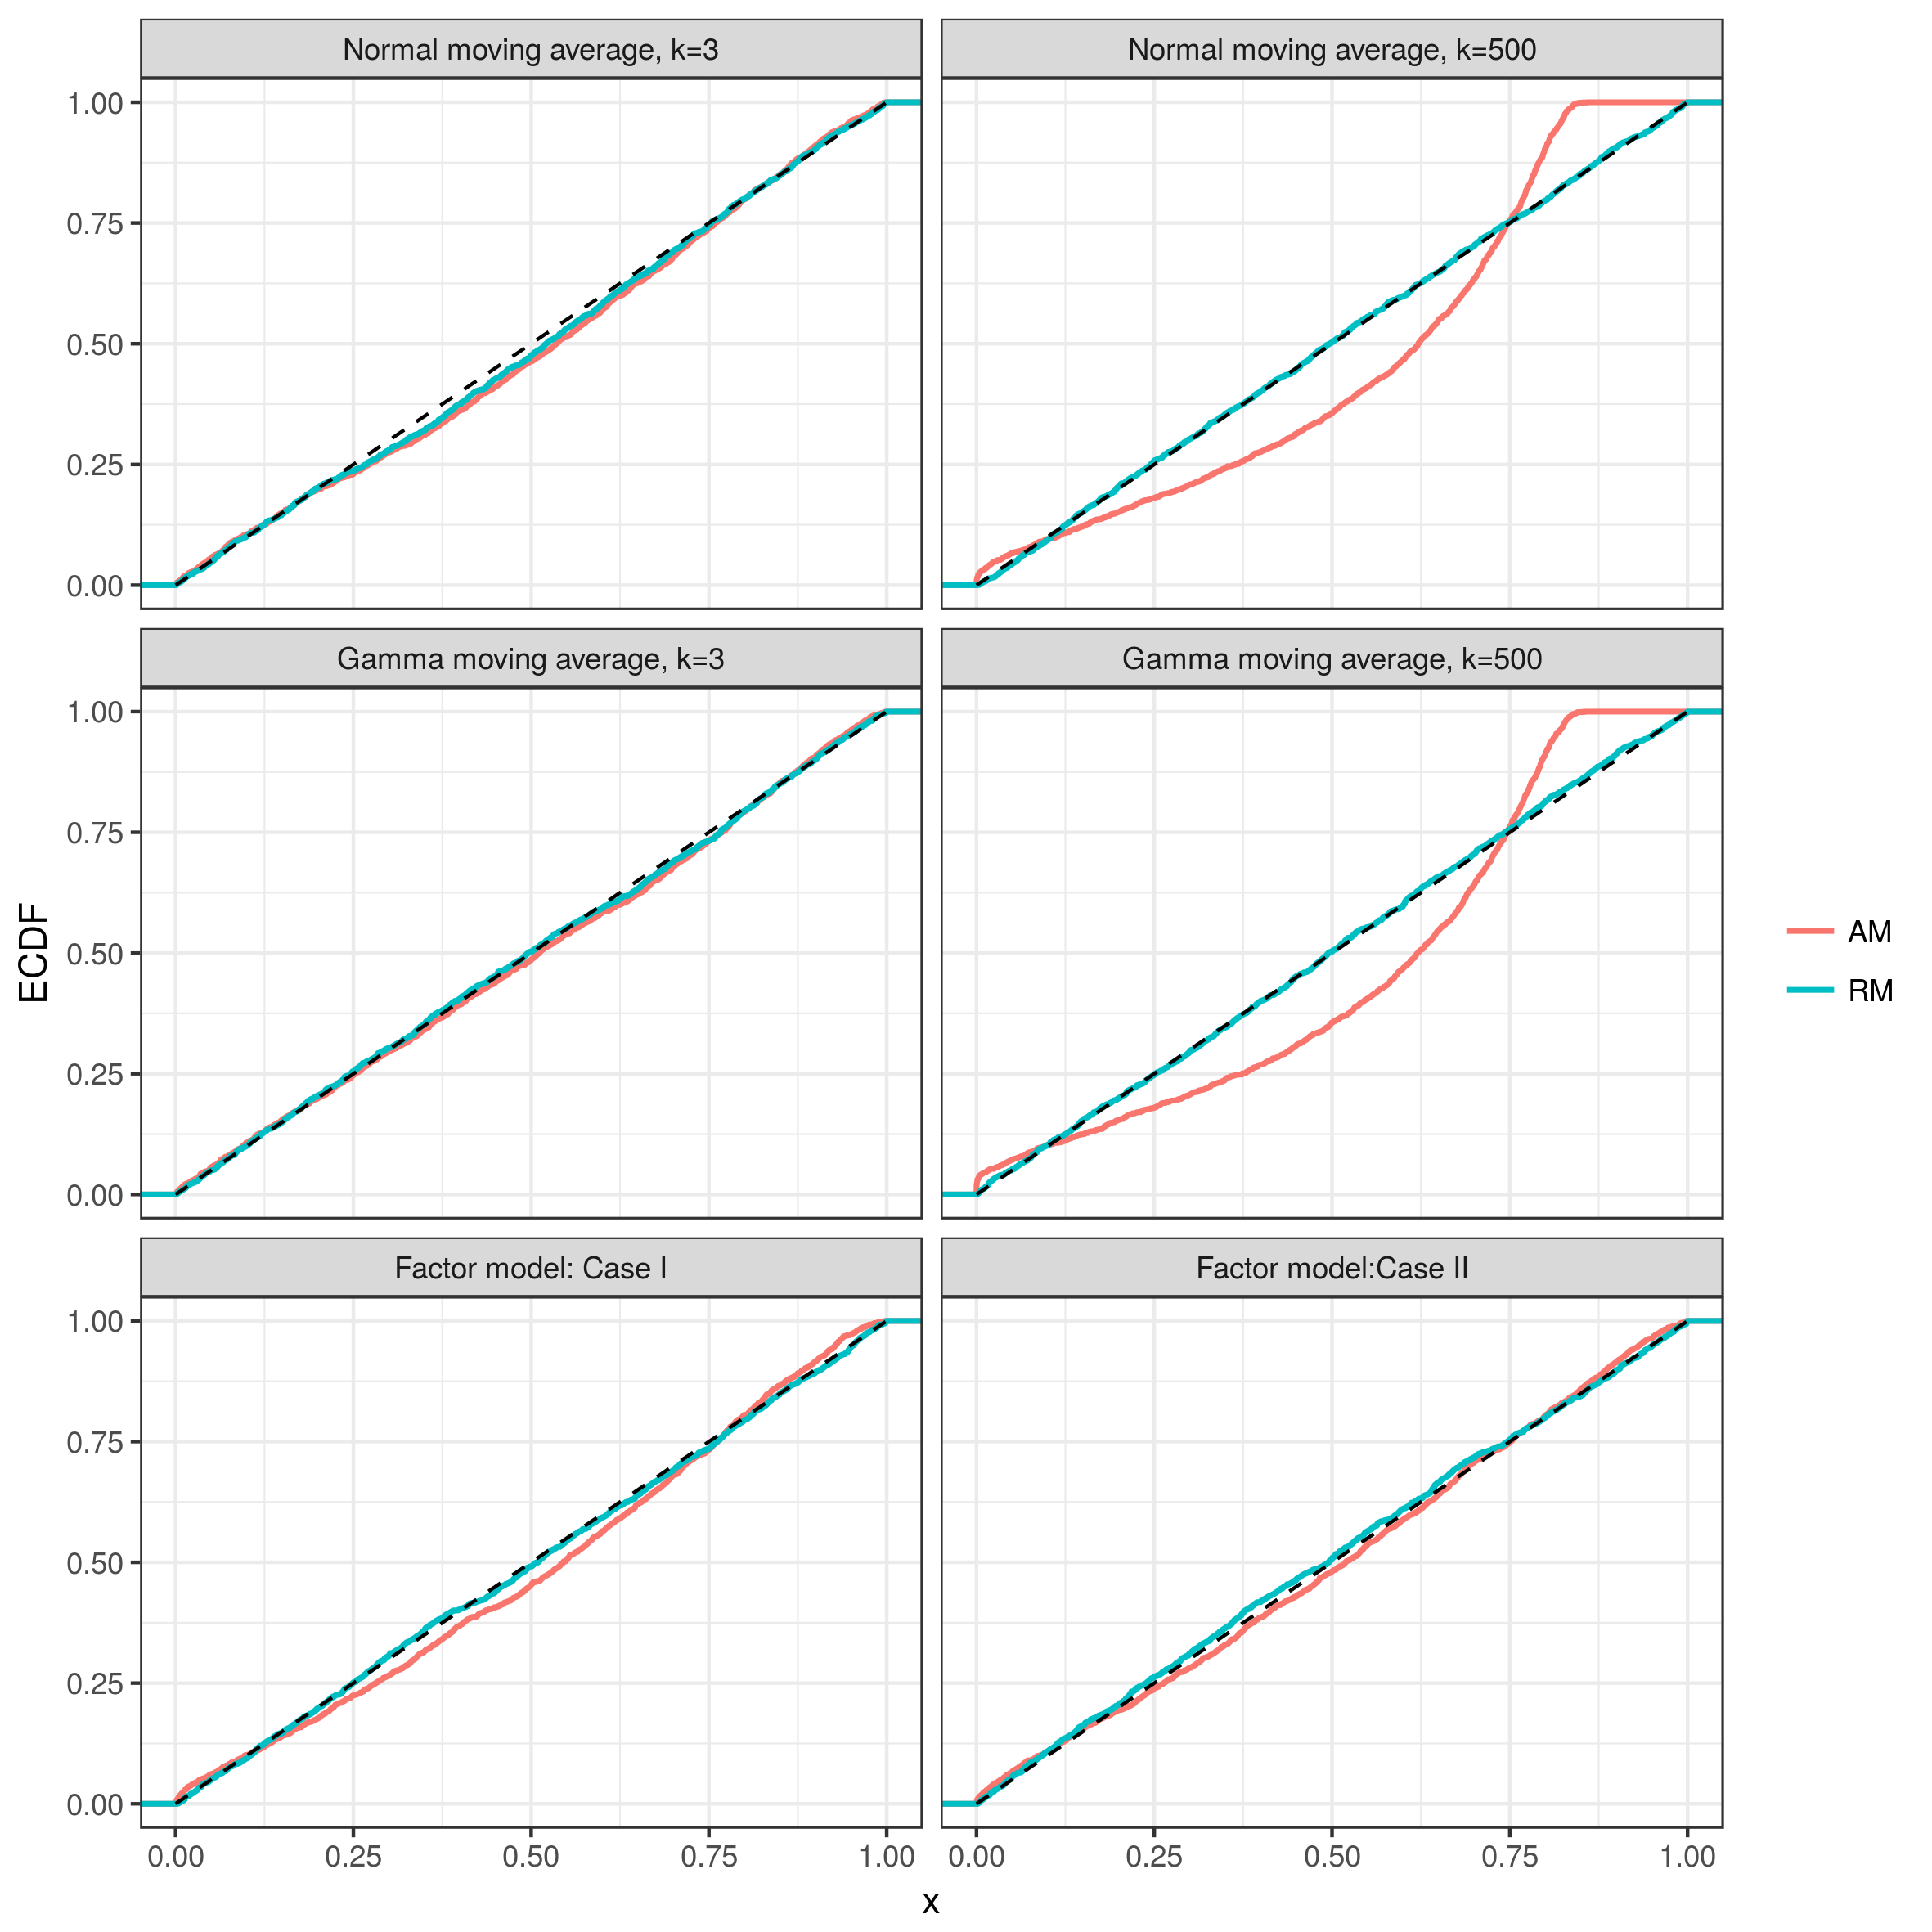
\includegraphics[width=12cm,height=12cm]{pValuePlotProposed.png}
    \caption{The ECDF of $p$-values for asymptotic method (AM) and randomization method (RM).  $p=600$, $n=100$.}\label{figure:ECDF}
\end{figure}

In Theorem~\ref{shaziCLT}, we proved that the randomization distribution tends to a standard normal distribution under certain conditions.
In Figure~\ref{figure:histogram}, we plot the histograms of randomization distribution under null hypothesis.
For comparison, we also plot the standard normal density.
From the plots, we can see that the randomization distribution is very similar to the standard normal distribution in factor model and moving average model with $k=3$.
This verifies our theorem~\ref{shazeCLT}.
However, under moving average model with $k=500$, the randomization distribution is far from standard normal distribution.
This implies the accuracy of normal approximation depends on the innovation model.


\begin{figure}[htbp]
    \centering
    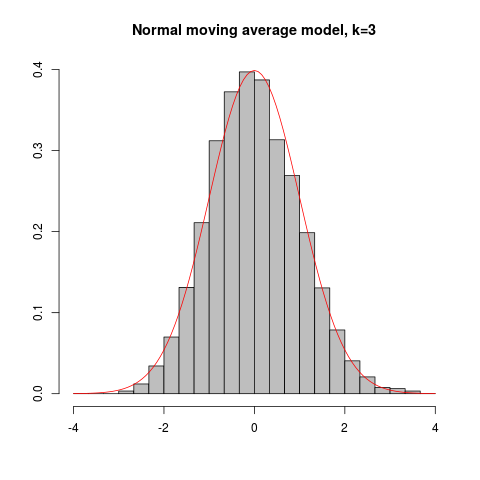
\includegraphics[width=6cm]{normal3.png}
    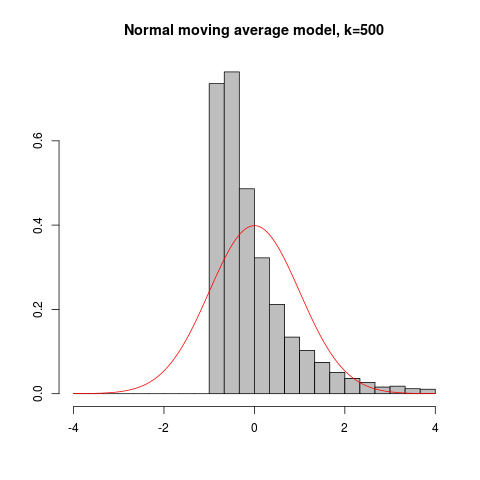
\includegraphics[width=6cm]{normal500.png}\\
    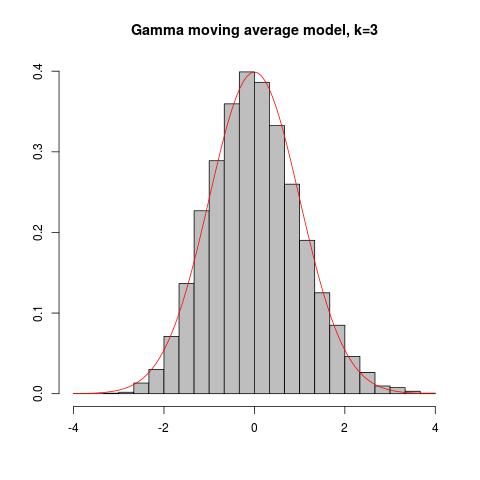
\includegraphics[width=6cm]{gamma3.png}
    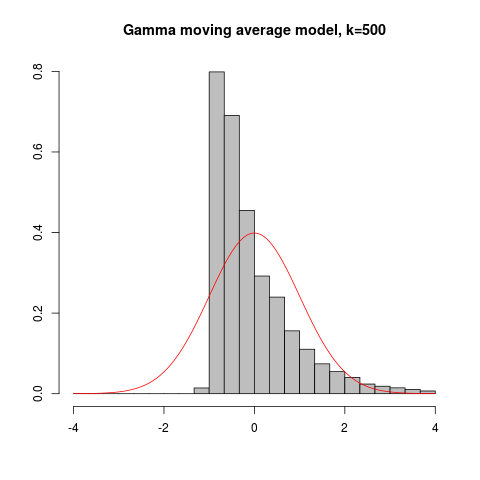
\includegraphics[width=6cm]{gamma500.png}\\
    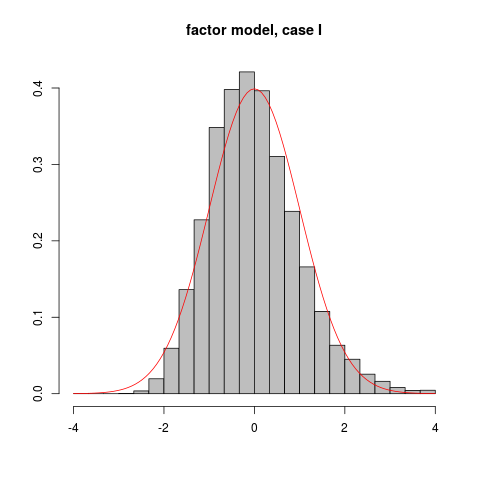
\includegraphics[width=6cm]{factor1.png}
    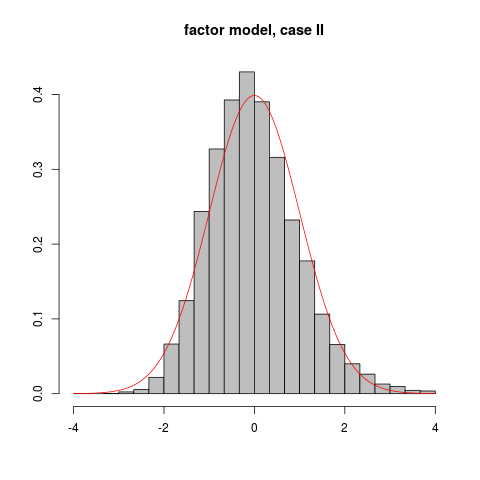
\includegraphics[width=6cm]{factor2.png}\\
    \caption{The histograms of the randomization distribution. $p=600$,$n=100$.}\label{figure:histogram}
\end{figure}




Now we simulate the empirical power and size.
Let $\mathrm{SNR}=\sqrt{n(n-1)}\mu^T \mu /\sqrt{2\mathrm{tr}\Sigma^2}$ be the signal to noise ratio (SNR).
The theoretic asymptotic power is an increasing function of SNR\@.
We scale $\mu$ to reach different level of SNR\@.
Our simulation consider two mean structure: dense mean and sparse mean.
In the dense mean setting, each coordinate of $\mu$ is independently generated from $U(2,3)$ and then $\mu$ is scaled to reach a given SNR\@.
In the sparse mean setting, we randomly select $5\%$ of $\mu$ $p$ coordinates to be non-zero.
Each non-zero coordinate is again independently generated from $U(2,3)$ and then scaled to reach a given SNR\@.
We set $B=1000$ for randomization test method.
The empirical power and size are computed based on $2000$ simulations.

Table~\ref{table1} and Table~\ref{table2} list the empirical power and size for the moving average model.
It's not surprising that randomization test can control level well in normal case since it can be proved in theory.
The results also show that the randomization method can control level well even in Gamma case, which is not symmetric under null.
It justifies the robustness of randomization method.
On the other hand, asymptotic method has small size when dependence is weak and has inflated size when dependence is strong.
Randomization method has similar power behavior with asymptotic method.
The empirical power of both methods is similar to theoretical asymptotic power~\eqref{oPower} while it is lower than theoretical asymptotic power when $k$ is large.
Table~\ref{table3} lists the empirical power and size under factor model.
Although the distribution is not symmetric, the results show that the level of randomization method is close to $0.05$ while asymptotic method suffers from level inflation.
In summary, the simulation results show that the randomization method is robust and has similar power with asymptotic method.

\begin{table}[ht]
    \footnotesize
    \caption{Empirical power and size of moving average model with normal innovation.  $p=600$, $n=100$, $\alpha=0.05$. TP is the theoretical asymptotic power, RM represents the randomization method, AM represents the asymptotic method.}
\label{table1}
    \centering
    \begin{tabular}{cccccccccc}
          \toprule
          & & \multicolumn{4}{c}{Dense means} &\multicolumn{4}{c}{Sparse means}\\
          \cmidrule(r){3-6}\cmidrule(r){7-10}
          & & \multicolumn{2}{c}{$k=3$} & \multicolumn{2}{c}{$k=500$} & \multicolumn{2}{c}{$k=3$}& \multicolumn{2}{c}{$k=500$}\\
          \cmidrule(r){3-4}  \cmidrule(r){5-6} \cmidrule(r){7-8}  \cmidrule(r){9-10}
           SNR& TP & RM & AM & RM & AM & RM & AM & RM & AM  \\ 
            \midrule
        0.0 & 0.050 & 0.0445 & 0.0515 & 0.0530 & 0.0745 & 0.0500 & 0.0585 & 0.0515 & 0.0715 \\ 
          0.5 & 0.126 & 0.1815 & 0.1940 & 0.1330 & 0.1685 & 0.1735 & 0.1875 & 0.0780 & 0.1130 \\ 
            1.0 & 0.260 & 0.4075 & 0.4295 & 0.2250 & 0.2785 & 0.4060 & 0.4325 & 0.1505 & 0.2065 \\ 
              1.5 & 0.442 & 0.6295 & 0.6535 & 0.3435 & 0.3920 & 0.6520 & 0.6755 & 0.2480 & 0.3355 \\ 
                2.0 & 0.639 & 0.7895 & 0.8055 & 0.3935 & 0.4665 & 0.8575 & 0.8765 & 0.3850 & 0.5400 \\ 
                  2.5 & 0.804 & 0.9165 & 0.9215 & 0.4775 & 0.5425 & 0.9655 & 0.9695 & 0.6355 & 0.8155 \\ 
                    3.0 & 0.912 & 0.9640 & 0.9695 & 0.5445 & 0.6090 & 0.9910 & 0.9935 & 0.8720 & 0.9730 \\ 
        \bottomrule
    \end{tabular}
\end{table}

\begin{table}[ht]
    \footnotesize
    \caption{Empirical power and size of moving average model with Gamma innovation.  $p=600$, $n=100$, $\alpha=0.05$. TP is the theoretical asymptotic power, RM represents the randomization method, AM represents the asymptotic method.}
\label{table2}
    \centering
    \begin{tabular}{cccccccccc}
          \toprule
          & & \multicolumn{4}{c}{Dense means} &\multicolumn{4}{c}{Sparse means}\\
          \cmidrule(r){3-6}\cmidrule(r){7-10}
          & & \multicolumn{2}{c}{$k=3$} & \multicolumn{2}{c}{$k=500$} & \multicolumn{2}{c}{$k=3$}& \multicolumn{2}{c}{$k=500$}\\
          \cmidrule(r){3-4}  \cmidrule(r){5-6} \cmidrule(r){7-8}  \cmidrule(r){9-10}
           SNR& TP & RM & AM & RM & AM & RM & AM & RM & AM \\ 
            \midrule
        0.0 & 0.050 & 0.0450 & 0.0550 & 0.0475 & 0.0660 & 0.0405 & 0.0465 & 0.0505 & 0.0765 \\ 
          0.5 & 0.126 & 0.1815 & 0.1975 & 0.1365 & 0.1750 & 0.1765 & 0.1870 & 0.0985 & 0.1345 \\ 
            1.0 & 0.260 & 0.3825 & 0.4050 & 0.2375 & 0.2765 & 0.4130 & 0.4335 & 0.1550 & 0.2070 \\ 
              1.5 & 0.442 & 0.6210 & 0.6465 & 0.2975 & 0.3490 & 0.6580 & 0.6745 & 0.2225 & 0.3135 \\ 
                2.0 & 0.639 & 0.8180 & 0.8325 & 0.3920 & 0.4450 & 0.8645 & 0.8800 & 0.3890 & 0.5340 \\ 
                  2.5 & 0.804 & 0.9115 & 0.9260 & 0.4900 & 0.5465 & 0.9635 & 0.9665 & 0.6280 & 0.8200 \\ 
                    3.0 & 0.912 & 0.9710 & 0.9765 & 0.5505 & 0.6085 & 0.9940 & 0.9945 & 0.8600 & 0.9740 \\ 
        \bottomrule
    \end{tabular}
\end{table}

\begin{table}[ht]
    \footnotesize
    \caption{Empirical power and size of factor model innovation.  $p=600$, $n=100$, $\alpha=0.05$. TP is the theoretical asymptotic power, RM represents the randomization method, AM represents the asymptotic method.}
\label{table3}
    \centering
    \begin{tabular}{cccccccccc}
          \toprule
          & & \multicolumn{4}{c}{Dense means} &\multicolumn{4}{c}{Sparse means}\\
          \cmidrule(r){3-6}\cmidrule(r){7-10}
          & & \multicolumn{2}{c}{Case I} & \multicolumn{2}{c}{Case II} & \multicolumn{2}{c}{Case I}& \multicolumn{2}{c}{Case II}\\
          \cmidrule(r){3-4}  \cmidrule(r){5-6} \cmidrule(r){7-8}  \cmidrule(r){9-10}
           SNR& TP & RM & AM & RM & AM & RM & AM & RM & AM  \\ 
            \midrule
        0.0 & 0.050 & 0.0465 & 0.0610 & 0.0455 & 0.0590 & 0.0475 & 0.0625 & 0.0505 & 0.0615 \\ 
          0.5 & 0.126 & 0.1315 & 0.1555 & 0.1465 & 0.1650 & 0.1200 & 0.1380 & 0.1080 & 0.1320 \\ 
            1.0 & 0.260 & 0.2420 & 0.2780 & 0.2550 & 0.2780 & 0.1940 & 0.2250 & 0.2075 & 0.2400 \\ 
              1.5 & 0.442 & 0.3635 & 0.3975 & 0.3555 & 0.3870 & 0.3670 & 0.4110 & 0.3740 & 0.4155 \\ 
                2.0 & 0.639 & 0.4825 & 0.5165 & 0.4720 & 0.4975 & 0.5340 & 0.5930 & 0.5615 & 0.6015 \\ 
                  2.5 & 0.804 & 0.5860 & 0.6190 & 0.5825 & 0.6165 & 0.7040 & 0.7610 & 0.7120 & 0.7505 \\ 
                    3.0 & 0.912 & 0.6730 & 0.7060 & 0.6975 & 0.7210 & 0.8525 & 0.8815 & 0.8680 & 0.8920 \\ 
        \bottomrule
    \end{tabular}
\end{table}

%\subsection{The second simulation study}
%The computation of our randomization test is easy since we only need to compute $X_i^T X_j$ once, $1\leq j<i \leq n$.
%The same technique can be applied to the statistic $\sum_{i\neq j}\|X_i\|^{-1}\|X_j\|^{-1}X_i^T X_j$ in~\cite{Wang2015A}.
%However, the technique can not be applied to the statistic $\bar{X}^T [\mydiag(S)]^{-1}\bar{X}$ in~\cite{Srivastava2008A} and the statistic $\bar{X}^T (I_p-\BP_S)\bar{X}$ in~\cite{Zhao2016A}.
%Generally, many high dimensional test statistics for hypotheses~\eqref{ourHy} can be written as generalized quadratic forms of data
%$$
%\sum_{i=1}^n \sum_{j=1}^n X_i^T A X_j,
%$$
%Where $A$ is a $p\times p$ matrix which only depends on $S$.
%The difficulty is that for each randomization, the matrix $A$ should be recalculated.
%It consumes a lot time.
%However, 
%the matrix $A$ is used to estimate the structure of $\Sigma$, which should not change during randomization.
%This motivates us to hold $A$ constant during randomization.
%More precisely, for a randomization, we generate $\epsilon_1,\ldots,\epsilon_n$ and compute
%$$
%\sum_{j<i} X_i^T A X_j \epsilon_i \epsilon_j.
%$$
%We simulate the level.
%
%We consider the following $A$:
%$A_1=[\mydiag(S)]^{-1}$,
%$A_2=\bar{X} S^{+}\bar{X}$,
%$A_3=(I-\BP_S)$,
%$A_4=S$.







\section{Conclusion Remark}
In this paper, we considered a randomization test for mean vector in high dimensional setting.
A fast implementation was provided.
We also derived some asymptotic properties of the test procedure.
For illustration, we only considered a special statistic. In fact, the algorithm and the proof method can be applied to other quadratic based statistics.

We showed that even if the symmetric assumption is violated, the randomization test also has correct level asymptotically.
Hence the test procedure is robust.
%It is interesting to investigate the robustness of randomization test in finite sample case.

In classical statistics, randomization test procedure is time consuming.
Nevertheless, our algorithm shows that the time complexity of randomization test procedure is not affected by dimension. 
The randomization test can be even more efficient than asymptotic method while holding desirable statistic properties.
Hence we have reason to believe that randomization tests may be generally suitable for high dimensional problems.


Maybe the most widely used randomization method is the two sample permutation test.
As~\cite{Romano1990On} pointed out, the asymptotic property of randomization tests depends heavily on the particular problem and the two sample case is quite distinct from the one sample case.
The method used in this paper can not be applied to permutation test.
We leave it for possible future work.


\section{Appendix}
\paragraph{A CLT for quadratic form of Rademacher variables}
The proof of the Theorem~\ref{shaziCLT} is based on a CLT of the quadratic form of Rademacher variables. 
Such a CLT can be also used to study the asymptotic behavior of many other randomization test.
 Let $\epsilon_1,\ldots,\epsilon_n$ be independent Rademacher  variables. 
 Consider quadratic form $W_n=\sum_{1\leq j<i\leq n} a_{ij}\epsilon_i \epsilon_j$, where $\{a_{ij}\}$ are nonrandom numbers. Here $\{\epsilon_i\}$ and $\{a_{ij}\}$ may depend on $n$, a parameter we suppress.
 Obviously, $\mathrm{E}(W_n)=0$ and $\mathrm{Var}(W_n)=\sum_{1\leq j<i\leq n} a_{ij}^2$.

 \begin{proposition}\label{CLTprop}
     A sufficient condition for
     \begin{equation*}
         \frac{W_n}{\sqrt{\sum_{1\leq j<i\leq n} a_{ij}^2}}\xrightarrow{\mathcal{L}} N(0,1)
     \end{equation*}
     is that
     \begin{equation*}
         \sum_{j<k}{(\sum_{i:i>k}a_{ij}a_{ik})}^2+
         \sum_{j<i}a_{ij}^4+
         \sum_{j<k<i}a_{ij}^2 a_{ik}^2
         =o\big({(\sum_{j<i} a_{ij}^2)}^2\big).
     \end{equation*}
 \end{proposition}

 \begin{proof}
     Define $U_{in} =\epsilon_i \sum_{j=1}^{i-1} a_{ij}\epsilon_j$, $i=2,\ldots,n$, and $\mathcal{F}_{in}=\sigma\{\epsilon_1,\ldots,\epsilon_i\}$, $i=1,\ldots, n$.
     Now $W_n=\sum_{i=2}^n U_{in}$, $\{U_{in}\}$ is a martingale difference array with respect to $\{\mathcal{F}_{in}\}$. 
Then MCLT can be used. See, for example,~\cite{pollard1984convergence}, Chapter VIII Theorem 1.
     To prove the proposition, we shall verify two conditions:
     \begin{equation}\label{MCLTcondition1}
         \frac{\sum_{i=2}^n \mathrm{E}(U_{in}^2 |\mathcal{F}_{i-1,n})}{\sum_{1\leq j<i\leq n} a_{ij}^2}\xrightarrow{P} 1,
     \end{equation}
     and
     \begin{equation}\label{MCLTcondition2}
         \frac{\sum_{i=2}^n \mathrm{E}\big(U_{in}^2\big\{U_{in}^2>\epsilon \sum_{1\leq j<i\leq n} a_{ij}^2\big\}\big|\mathcal{F}_{i-1,n}\big)}{\sum_{1\leq j<i\leq n} a_{ij}^2}\xrightarrow{P} 0,
     \end{equation}
     for every $\epsilon>0$.

     \paragraph{Proof of~\eqref{MCLTcondition1}}
     Since $\mathrm{E}(U_{in}^2 |\mathcal{F}_{i-1,n})={(\sum_{j=1}^{i-1}a_{ij}\epsilon_j)}^2$, we have
     \begin{equation*}
         \begin{aligned}
\sum_{i=2}^n \mathrm{E}(U_{in}^2 |\mathcal{F}_{i-1,n})
             &=\sum_{i=2}^n \big(\sum_{j=1}^{i-1}a_{ij}\epsilon_j \big)^2
             =\sum_{i=2}^n \big( \sum_{j=1}^{i-1} a_{ij}^2 +2\sum_{j,k:j<k<i} a_{ij}a_{ik}\epsilon_j \epsilon_k \big)\\
             &=\sum_{i=2}^n  \sum_{j=1}^{i-1} a_{ij}^2 +2\sum_{j<k<i} a_{ij}a_{ik}\epsilon_j \epsilon_k.
         \end{aligned}
     \end{equation*}

     But
     \begin{equation*}
         \begin{aligned}
         \mathrm{E}{(\sum_{j<k<i} a_{ij}a_{ik}\epsilon_j \epsilon_k)}^2
             &=
             \mathrm{E}{\big(\sum_{j<k} (\sum_{i:i>k}a_{ij}a_{ik})\epsilon_j \epsilon_k \big)}^2\\
             &=
             \sum_{j<k} (\sum_{i:i>k}a_{ij}a_{ik})^2
             =
             o\big({(\sum_{j<i} a_{ij}^2)}^2\big),
         \end{aligned}
     \end{equation*}
     where the last equality holds by assumption. Hence~\eqref{MCLTcondition1} holds.
     \paragraph{Proof of~\eqref{MCLTcondition2}}
     By Markov's inequality, we only need to prove
     \begin{equation}\label{temp1}
         \frac{\sum_{i=2}^n \mathrm{E}\big(U_{in}^4\big|\mathcal{F}_{i-1,n}\big)}{{\big(\sum_{1\leq j<i\leq n} a_{ij}^2\big)}^2}\xrightarrow{P} 0.
     \end{equation}
     Since the relevant random variables are all positive, we only need to prove~\eqref{temp1} converges to $0$ in mean. But
     \begin{equation*}
         \begin{aligned}
         \sum_{i=2}^n \mathrm{E} U_{in}^4
             &=
             \sum_{i=2}^n \mathrm{E} {(\sum_{j:j<i}a_{ij}\epsilon_j)}^4
             =
             \sum_{i=2}^n \mathrm{E} {(\sum_{j:j<i}a_{ij}^2+2\sum_{j,k:j<k<i}a_{ij}a_{ik}\epsilon_j \epsilon_k)}^2\\
             &=
             \sum_{i=2}^n  \big({(\sum_{j:j<i}a_{ij}^2)}^2+4\mathrm{E}{(\sum_{j,k:j<k<i}a_{ij}a_{ik}\epsilon_j \epsilon_k)}^2 \big)\\
             &=
             \sum_{i=2}^n  (\sum_{j:j<i}a_{ij}^4+6\sum_{j,k:j<k<i}a_{ij}^2 a_{ik}^2)\\
             &=
             \sum_{j<i}a_{ij}^4+6\sum_{j<k<i}a_{ij}^2 a_{ik}^2
             =
             o\big({(\sum_{j<i} a_{ij}^2)}^2\big),
         \end{aligned}
     \end{equation*}
     where the last equality holds by assumption. Hence~\eqref{MCLTcondition2} holds.
 \end{proof}

 The rest of Appendix is devoted to the proof of the theorems in the paper.


\begin{lemma}\label{lemmaUniformSimple}
    Suppose $\{\eta_n\}$ is a sequence of $1$-dimensional random variables, weakly converges to $\eta$, a random variable with continuous distribution function.
    Then we have
    $$
    \sup_{x}|\Pr(\eta_n\leq x)-\Pr(\eta\leq x)|\to 0.
    $$
\end{lemma}

\begin{lemma}\label{lemmaQ}
    Suppose $A=(a_{ij})$ is an $m\times m$ positive semi-definite matrix. Under~\eqref{chenC2}, we have
        $$
        \mathrm{E} {(Z_i^T A Z_i)}^2\asymp {(\mathrm{tr}A)}^2
        $$
\begin{proof}
Notice that
    $$
    \begin{aligned}
        {(Z_i^T A Z_i)}^2
        =&
        (\sum_{j=1}^m a_{jj}z_{ij}^2+2\sum_{k<j}a_{jk}z_{ij}z_{ik})^2\\
        =&
        (\sum_{j=1}^m a_{jj}z_{ij}^2)^2+
        4(\sum_{j=1}^m a_{jj}z_{ij}^2)(\sum_{k<j}a_{jk}z_{ij}z_{ik})+
        4(\sum_{k<j}a_{jk}z_{ij}z_{ik})^2\\
        =&
        \sum_{j=1}^m a_{jj}^2z_{ij}^4+2\sum_{k<j}a_{jj}a_{kk}z_{ij}^2 z_{ik}^2+
        4(\sum_{j=1}^m a_{jj}z_{ij}^2)(\sum_{k<j}a_{jk}z_{ij}z_{ik})\\
        &+
        4(\sum_{k<j}a_{jk}^2z_{ij}^2z_{ik}^2+\sum_{k<j,l<\alpha:\mathrm{card}(\{k,j\}\cap\{l,\alpha\})<2} a_{jk}a_{\alpha l}z_{ij}z_{ik}z_{i\alpha}z_{il})\\
    \end{aligned}
    $$
Hence
    $$
    \begin{aligned}
        \mathrm{E}{(Z_i^T A Z_i)}^2
        =&
        \sum_{j=1}^n a_{jj}^2 \mathrm{E}z_{ij}^4+2\sum_{k<j}a_{jj}a_{kk}\mathrm{E}(z_{ij}^2 z_{ik}^2)+
        4\sum_{k<j}a_{jk}^2 \mathrm{E}(z_{ij}^2z_{ik}^2)\\
        \asymp &
        \sum_{j=1}^n\sum_{k=1}^n a_{jj}a_{kk}+
        \sum_{j=1}^n\sum_{k=1}^n a_{jk}^2
        ={(\mathrm{tr}(A))}^2+\mathrm{tr}A^2.
    \end{aligned}
    $$

    By Cauchy inequality, $0\leq \mathrm{tr} A^2\leq {(\mathrm{tr}A)}^2$. The conclusion holds.

\end{proof}
\end{lemma}

\begin{lemma}\label{smallLemma1}
    Under~\eqref{chenC1},~\eqref{chenC2}, for $i\neq j$ we have
    \begin{equation}\label{eq:20170220}
        \mathrm{E}{(X_i^T X_j)}^4=%O\Big({\big(\mathrm{tr}(\Sigma+\mu\mu^T)^2\big)}^2\Big).
             O(1){\Big(\mathrm{tr}{\big(\Sigma+\mu\mu^T\big)}^2\Big)}^2.
    \end{equation}
\end{lemma}
\begin{proof}
    $$
        \begin{aligned}
            {(X_i^T X_j)}^4=&
            {(Z_i^T \Gamma^T \Gamma Z_j+\mu^T \Gamma Z_i+\mu^T \Gamma Z_j+\mu^T \mu)}^4\\
            \leq &
            64\big((Z_i^T \Gamma^T \Gamma Z_j)^4+(\mu^T \Gamma Z_i)^4+(\mu^T \Gamma Z_j)^4+(\mu^T \mu)^4\big)\\
        \end{aligned}
    $$
    We deal with the first term by applying Lemma~\ref{lemmaQ} twice.
        $$
        \begin{aligned}
            \mathrm{E}(Z_i^T \Gamma^T \Gamma Z_j)^4=&
        \mathrm{E}(Z_i^T \Gamma^T \Gamma Z_j Z_j^T \Gamma^T \Gamma Z_i)^2
            =
            \mathrm{E}\mathrm{E}\big((Z_i^T \Gamma^T \Gamma Z_j Z_j^T \Gamma^T \Gamma Z_i)^2 | Z_j\big)\\
            \asymp &  \mathrm{E}{(Z_j^T \Gamma^T \Sigma \Gamma Z_j)}^2
            \asymp   {(\mathrm{tr}\Sigma^2)}^2,%+\mathrm{tr}\Sigma^4\\
            %\leq &  (\mathrm{tr}\Sigma^2)^2+\lambda_{\max}^2(\Sigma)\mathrm{tr}\Sigma^2,
        \end{aligned}
    $$
    Similarly, we have
        $$
        \begin{aligned}
            &\mathrm{E}(\mu^T \Gamma Z_i)^4=
        \mathrm{E}(Z_i^T \Gamma^T \mu\mu^T \Gamma Z_i)^2
            \asymp  {(\mu^T \Sigma \mu)}^2\\
            &\leq \lambda_{\max}^2(\Sigma){(\mu^T \mu)}^2
        \leq \mathrm{tr}(\Sigma^2){(\mu^T \mu)}^2
            \leq {\big(\mathrm{tr}(\Sigma^2)\big)}^2+{(\mu^T \mu)}^4.
        %\leq \lambda_{\max}^2(\Sigma){(\mu^T\mu)}^2
        \end{aligned}
    $$
    Thus, the conclusion holds.
\end{proof}


\begin{lemma}\label{smallLemma2}
    Under~\eqref{chenC1},~\eqref{chenC2}, suppose $i\neq j$, $i\neq k$, $j\neq k$, we have
    \begin{equation}\label{eq:2}
            \mathrm{E}{(X_i^T X_j)}^2{(X_k^T X_i)}^2=
             O(1){\Big(\mathrm{tr}{\big(\Sigma+\mu\mu^T\big)}^2\Big)}^2.
    \end{equation}
\end{lemma}
\begin{proof}
Note that
    \begin{equation*}
        \begin{aligned}
            &\mathrm{E}{(X_i^T X_j)}^2{(X_k^T X_i)}^2
            = 
            \mathrm{E}\mathrm{E}\big({(X_i^T X_j)}^2{(X_k^T X_i)}^2| X_i\big)
            =
            \mathrm{E}{(X_i^T (\Sigma+\mu\mu^T) X_i )}^2\\
            =&
            \mathrm{E}{\big(Z_i^T \Gamma^T (\Sigma+\mu\mu^T) \Gamma Z_i+ 2\mu^T (\Sigma+\mu\mu^T)\Gamma Z_i +\mu \Sigma \mu +(\mu^T\mu)^2 \big)}^2\\
            \leq&
            4\mathrm{E}(Z_i^T \Gamma^T (\Sigma+\mu\mu^T) \Gamma Z_i)^2+ 16\mathrm{E}(\mu^T (\Sigma+\mu\mu^T)\Gamma Z_i)^2 +4(\mu \Sigma \mu)^2 +4(\mu^T\mu)^4.
        \end{aligned}
    \end{equation*}
    By Lemma~\eqref{lemmaQ},
    \begin{equation*}
        \begin{aligned}
\mathrm{E}(Z_i^T \Gamma^T (\Sigma+\mu\mu^T) \Gamma Z_i)^2
            &\asymp
\big(\mathrm{tr}(\Gamma^T (\Sigma+\mu\mu^T)\Gamma)\big)^2\\
            &=
\big(\mathrm{tr}\Sigma^2+\mu^T\Sigma \mu\big)^2
            \leq
            2{\big(\mathrm{tr}\Sigma^2\big)}^2+2{\big(\mu^T\Sigma \mu\big)}^2.
        \end{aligned}
    \end{equation*}
    And
    \begin{equation*}
        \begin{aligned}
            &\mathrm{E}(\mu^T (\Sigma+\mu\mu^T)\Gamma Z_i)^2=
\mu^T (\Sigma+\mu\mu^T)\Sigma (\Sigma+\mu\mu^T)\mu\\
            =&\mu^T \Sigma^3 \mu+2(\mu^T\mu)(\mu^T\Sigma^2\mu)+{(\mu^T\mu)}^2(\mu^T\Sigma\mu).
        \end{aligned}
    \end{equation*}

    But for $i=1,2,\ldots$, we have
    $$
    \mu^T \Sigma^i \mu
    \leq \lambda_{\max}^i(\Sigma)\mu^T\mu
    \leq {(\mathrm{tr}(\Sigma^2))}^{i/2}\mu^T\mu.
    $$
    Thus,
        $$
        \begin{aligned}
            &\mathrm{E}{(X_i^T X_j)}^2{(X_k^T X_i)}^2\\
            =&
            O(1)\big({(\mathrm{tr}\Sigma^2)}^2+
            {(\mathrm{tr}\Sigma^2)}^{3/2}{(\mu^T \mu)}+
            {(\mathrm{tr}\Sigma^2)}{(\mu^T \mu)}^2+
            {(\mathrm{tr}\Sigma^2)}^{1/2}{(\mu^T \mu)}^3+
            {(\mu^T \mu)}^4
            \big)\\
            =& O(1){\Big(\mathrm{tr}{\big(\Sigma+\mu\mu^T\big)}^2\Big)}^2.
        \end{aligned}
        $$
\end{proof}


\begin{lemma}\label{ratioLemma}
    Under~\eqref{chenC1} and~\eqref{chenC2}, we have
        $$
        \frac{\sum_{j<i}{(X_i^T X_j)}^2}{\frac{n(n-1)}{2}\mathrm{tr} (\Sigma+\mu\mu^T)^2}
        \xrightarrow{P}1.
        $$
\end{lemma}
\begin{proof}
    Since
        $$
        \begin{aligned}
            \mathrm{E}{(X_i^T X_j)}^2=&
            \mathrm{E}(X_i^T X_j X_j^T X_i)=
            \mathrm{E}(X_i^T (\Sigma+\mu \mu^T) X_i)\\
            =&
            \mathrm{E}\mathrm{tr}((\Sigma+\mu \mu^T) X_i X_i^T)=\mathrm{tr}{(\Sigma+\mu \mu^T)}^2,
        \end{aligned}
    $$
   we have 
        $$
        \mathrm{E}\sum_{j<i}{(X_i^T X_j)}^2=\frac{n(n-1)}{2}\mathrm{tr}{(\Sigma+\mu\mu^T)}^2
    $$
    So we only need to consider the variance. According to $\mathrm{card}(\{i,j\}\cap\{k,l\})=0,1,2$, we have
    \begin{equation}\label{eq:1}
    \begin{aligned}
        &{\big(\sum_{j<i}{(X_i^T X_j)}^2\big)}^2
        =
        \sum_{j<i}{(X_i^T X_j)}^4+
        \sum_{j<i,k<l:\{i,j\}\cap \{k,l\}=\phi}{(X_i^T X_j)}^2{(X_k^T X_l)}^2\\
        &+2\sum_{j<i<k}\big(
        {(X_i^T X_j)}^2{(X_k^T X_i)}^2+
{(X_i^T X_j)}^2{(X_k^T X_j)}^2+
{(X_k^T X_j)}^2{(X_k^T X_i)}^2
        \big).
    \end{aligned}
    \end{equation}


   
    In~\eqref{eq:1}, there are $n(n-1)/2$, $n(n-1)(n-2)(n-3)/4$ and $n(n-1)(n-2)/6$ terms in each summation. By Lemma~\ref{smallLemma1} and Lemma~\ref{smallLemma2}, we have
    $$
    \begin{aligned}
        \mathrm{E}{\big(\sum_{j<i}{(X_i^T X_j)}^2\big)}^2
            =&\frac{n(n-1)(n-2)(n-3)}{4}{\big(\mathrm{tr}(\Sigma+\mu\mu^T)^2\big)}^2\\
            &+O(1)(\frac{n(n-1)}{2}+n(n-1)(n-2)){\big(\mathrm{tr}(\Sigma+\mu\mu^T)^2\big)}^2.
    \end{aligned}
    $$
Hence 
    $$
    \frac{
        \mathrm{Var}(\sum_{j<i}{(X_i^T X_j)}^2)
    }{\big(\mathrm{E}\sum_{j<i}{(X_i^T X_j)}^2\big)^2}
    =
    \frac{
        \mathrm{E}{\big(\sum_{j<i}{(X_i^T X_j)}^2\big)}^2-
        {\big(\mathrm{E}\sum_{j<i}{(X_i^T X_j)}^2\big)}^2
    }{
        {\big(\mathrm{E}\sum_{j<i}{(X_i^T X_j)}^2\big)}^2
    }
    =O(\frac{1}{n}).
    $$
    Thus the conclusion holds.
\end{proof}

\begin{lemma}
    Under~\eqref{chenC1},~\eqref{chenC2},~\eqref{chenC3} and 
    \begin{equation}\label{myLoc}
        \mu^T \mu=o(\sqrt{\mathrm{tr}\Sigma^2}),
    \end{equation}
we have
    \begin{equation}\label{lemma2R1}
        \sum_{j<k}{(\sum_{i:i>k}X_i^T X_j X_i^T X_k)}^2
        =o_P\Big(\big(\frac{n(n-1)}{2}\mathrm{tr}(\Sigma+\mu\mu^T)^2\big)^2\Big).
    \end{equation}
    \begin{equation}\label{lemma2R2}
        \sum_{j<k}{(X_i^T X_j)}^4=o_P\Big(\big(\frac{n(n-1)}{2}\mathrm{tr}(\Sigma+\mu\mu^T)^2\big)^2\Big)
    \end{equation}
    \begin{equation}\label{lemma2R3}
        \sum_{j<k<i}{(X_i^T X_j)}^2{(X_i^T X_k)}^2 =o_P\Big(\big(\frac{n(n-1)}{2}\mathrm{tr}(\Sigma+\mu\mu^T)^2\big)^2\Big)
    \end{equation}
\end{lemma}
\begin{proof}
    \begin{equation*}
    \begin{aligned}
        &\mathrm{E}\sum_{j<k}{(\sum_{i:i>k}X_i^T X_j X_i^T X_k)}^2\\
        =&
        \mathrm{E}\sum_{j<k}\Big(\sum_{i:i>k}(X_i^T X_j)^2 (X_i^T X_k)^2+2\sum_{i_1,i_2:i_1>i_2>k}X_{i_1}^T X_j X_{i_1}^T X_k X_{i_2}^T X_j X_{i_2}^T X_k\Big).\\
    \end{aligned}
    \end{equation*}

    By Lemma~\ref{smallLemma1}, we have
    \begin{equation*}
    \begin{aligned}
        \mathrm{E}\sum_{j<k<i}(X_i^T X_j)^2 (X_i^T X_k)^2    =O(n^3)\big(\mathrm{tr}(\Sigma+\mu\mu^T)^2\big)^2.
    \end{aligned}
    \end{equation*}
And
    \begin{equation*}
    \begin{aligned}
        &\mathrm{E}\sum_{j<k<i_2<i_1}X_{i_1}^T X_j X_{i_1}^T X_k X_{i_2}^T X_j X_{i_2}^T X_k\\
        =&\frac{n(n-1)(n-2)(n-3)}{6}\mathrm{tr}{(\Sigma+\mu\mu^T)}^4\\
        \leq& \frac{n(n-1)(n-2)(n-3)}{6}8(\mathrm{tr}{(\Sigma)}^4+(\mu^T \mu)^4)\\
        \leq& O(n^4)(\lambda_{\max}^2(\Sigma)\mathrm{tr}{(\Sigma)}^2+(\mu^T \mu)^4)\\
        =&
        o\Big(n^4{\big(\mathrm{tr}\Sigma^2\big)}^2\Big),
    \end{aligned}
    \end{equation*}
    where the last line follows by assumption~\eqref{chenC3} and~\eqref{myLoc}.
    Thus~\eqref{lemma2R1} holds.~\eqref{lemma2R2} and~\eqref{lemma2R3} follow by Lemma~\ref{smallLemma1} and Lemma~\ref{smallLemma2}.

\end{proof}

\begin{proof}[Proof of Theorem~\ref{shaziCLT}]
By a standard subsequence argument, we only need to prove 
    \begin{equation}\label{changchuan}
        \rho\Big(\mathcal{L}\Big(\frac{T_2(\epsilon_1 X_1,\ldots, \epsilon_i X_i,\ldots,\epsilon_n X_n)}{\sqrt{\sum_{1\leq j<i\leq n}{(X_i^T X_j)}^2}}\Big|X_1,\ldots,X_n\Big),N(0,1)\Big)\xrightarrow{a.s.} 0
    \end{equation}
     along a subsequence.
    But there is a subsequence $\{n(k)\}$ along which~\eqref{lemma2R1},~\eqref{lemma2R2} and~\eqref{lemma2R3} holds almost surely.
    By Proposition~\ref{CLTprop}, we have
    \begin{equation*}
        \mathcal{L}\Big(\frac{T_2(\epsilon_1 X_1,\ldots, \epsilon_i X_i,\ldots,\epsilon_n X_n)}{\sqrt{\sum_{1\leq j<i\leq n}{(X_i^T X_j)}^2}}\Big|X_1,\ldots,X_n\Big)\xrightarrow{\mathcal{L}}N(0,1)
    \end{equation*}
    almost surely along $\{n(k)\}$, which means~\eqref{changchuan} holds along $\{n(k)\}$.

\end{proof}

\begin{proof}[Proof of Theorem~\ref{farT}]
    \begin{equation*}
        \begin{aligned}
            \sum_{j<i} X_i^T X_j \epsilon_i\epsilon_j=&
            \sum_{j<i} Z_i^T \Gamma^T \Gamma Z_j \epsilon_i\epsilon_j\\
            &+
            \sum_{j<i} \mu^T \Gamma Z_i \epsilon_i\epsilon_j
            +\sum_{j<i} \mu^T \Gamma Z_j \epsilon_i\epsilon_j+
            \mu^T \mu \sum_{j<i} \epsilon_i\epsilon_j\\
            \overset{def}{=}&C_1+C_2+C_3+C_4.
        \end{aligned}
    \end{equation*}
Term $C_4$ plays a major role. Note that
    \begin{equation*}
        \begin{aligned}
            C_4=\frac{n}{2}\mu^T \mu\Big({\Big(\frac{1}{\sqrt{n}}\sum_{i=1}^n \epsilon_i\Big)}^2-1\Big).
        \end{aligned}
    \end{equation*}
By central limit theorem, we have
    \begin{equation*}
        \begin{aligned}
            \rho\Big(\mathcal{L}\Big(\frac{C_4}{\frac{n}{2}\mu^T \mu}\Big| X_1,\ldots,X_n\Big),\chi^2_1-1\Big)\xrightarrow{a.s.} 0.
        \end{aligned}
    \end{equation*}
Next we show that $C_1$, $C_2$ and $C_3$ are negligible under the assumptions of the theorem.
    By a standard subsequence argument and Slutsky's theorem, we can obtain
    \begin{equation}\label{rush2}
        \begin{aligned}
            \rho\Big(\mathcal{L}\Big(\frac{T(\epsilon_1 X_1,\ldots, \epsilon_i X_i,\ldots,\epsilon_n X_n)}{\frac{n}{2}\mu^T \mu}\Big| X_1,\ldots,X_n\Big),\chi^2_1-1\Big)\xrightarrow{P} 0
        \end{aligned}
    \end{equation}
    by showing that
    $$
    \mathrm{E}\Big({\Big(\frac{C_i}{\frac{n}{2}\mu^T\mu}\Big)}^2\Big|X_1,\ldots,X_n\Big)\xrightarrow{P} 0,\quad i=1,2,3.
    $$
    It in turn suffices to show

    \begin{equation}\label{Rush}
    \mathrm{E}{\Big(\frac{C_i}{\frac{n}{2}\mu^T\mu}\Big)}^2\to 0,
    \quad i=1,2,3.
    \end{equation}
    By direct calculation, we have
    $$\mathrm{E}(C_1^2)=\mathrm{E}\mathrm{E}(C_1^2|X_1,\ldots,X_n)=\sum_{j<i}\mathrm{E}{(Z_i^T \Gamma^T \Gamma Z_j)}^2=\frac{n(n-1)}{2}\mathrm{tr}\Sigma^2,$$
    and
    $$\mathrm{E}(C_2^2)=\mathrm{E}(C_3^2)=\frac{n(n-1)}{2}\mu^T \Sigma \mu\leq \frac{n(n-1)}{2}\sqrt{\mathrm{tr}\Sigma^2}\mu^T\mu.$$
    Thus~\eqref{Rush} follows by Assumption~\eqref{mu3}. Having~\eqref{rush2} holds, the theorem follows by Slutsky's theorem, Lemma~\ref{ratioLemma} and Assumption~\eqref{mu3}.
\end{proof}


\begin{proof}[\textbf{Proof of Corollaries~\ref{corollaryQuan} and~\ref{corollaryQuan2}}]
    For every subsequence, there is a further subsequence along which
    \begin{equation*}
        \rho\Big(\mathcal{L}\Big(\frac{T_2(\epsilon_1 X_1,\ldots, \epsilon_i X_i,\ldots,\epsilon_n X_n)}{\sqrt{\sum_{1\leq j<i\leq n}{(X_i^T X_j)}^2}}\Big|X_1,\ldots,X_n\Big),N(0,1)\Big)\to 0
    \end{equation*}
    almost surely.
    By the property of weak convergence, $\xi^*_\alpha\to \Phi(1-\alpha)$ almost surely along this subsequence.
That is, For every subsequence, there is a further subsequence along which $\xi^*_\alpha\to \Phi(1-\alpha)$ almost surely.
    This is equivalent to $\xi_{\alpha}^* \xi \xrightarrow{P}\Phi(1-\alpha)$.
    The proof of Corollary~\ref{corollaryQuan2} is similar.

\end{proof}

\begin{proof}[Proof of Theorem~\ref{theoremPower}]
    Note that
    \begin{align}
            &\Pr\Big(\frac{T( X_1,\ldots, X_n)}{\sqrt{\sum_{1\leq j<i\leq n}{(X_i^T X_j)}^2}}>\xi_{\alpha}^* \Big)\nonumber\\
            =&
            \Pr\Big(\frac{T( X_1,\ldots, X_n)-\frac{n(n-1)}{2}\mu^T\mu}{\sqrt{\sum_{1\leq j<i\leq n}{(X_i^T X_j)}^2}}>\xi_{\alpha}^*-\frac{\frac{n(n-1)}{2}\mu^T\mu}{\sqrt{\sum_{1\leq j<i\leq n}{(X_i^T X_j)}^2}} \Big)
            \label{powerEq1}
    \end{align}
    If~\eqref{mu2} holds, by Lemma~\ref{ratioLemma}, we have
    $$
    \frac{\sum_{1\leq j< i\leq n}(X_i^T X_j)^2}{\frac{n(n-1)}{2}\mathrm{tr}\Sigma^2}\xrightarrow{P}1.
    $$
    By Corollary~\ref{corollaryQuan}, we have $\xi_{\alpha}^*\xrightarrow{P} \Phi(1-\alpha)$.
Thus,
    \begin{equation*}
        \begin{aligned}
            \eqref{powerEq1}=&
            \Pr\Big(\frac{T( X_1,\ldots, X_n)-\frac{n(n-1)}{2}\mu^T\mu}{\sqrt{\frac{n(n-1)}{2}\mathrm{tr}\Sigma^2}}-
            \frac{\sqrt{\sum_{1\leq j<i\leq n}{(X_i^T X_j)}^2}}{\sqrt{\frac{n(n-1)}{2}\mathrm{tr}\Sigma^2}}\xi_{\alpha}^*>
            -\frac{\sqrt{n(n-1)}\mu^T\mu}{\sqrt{2\mathrm{tr}\Sigma^2}} \Big)\\
            =&
            \Pr\Big(N(0,1)-\Phi(1-\alpha)>-\frac{\sqrt{n(n-1)}\mu^T\mu}{\sqrt{2\mathrm{tr}\Sigma^2}}\Big)+o(1)\\
            =&
            \Phi(-\Phi(1-\alpha)+\frac{\sqrt{n(n-1)}\mu^T\mu}{\sqrt{2\mathrm{tr}\Sigma^2}})+o(1),
        \end{aligned}
    \end{equation*}
    where the last two equality holds by Theorem~\ref{theoremChen}, Slutsky's theorem and Lemma~\ref{lemmaUniformSimple}.

    If~\eqref{mu3} holds, by Lemma~\ref{ratioLemma}, we have
    $$
    \frac{\sum_{1\leq j< i\leq n}(X_i^T X_j)^2}{\frac{n(n-1)}{2}{(\mu^T\mu)}^2}\xrightarrow{P}1.
    $$
    Thus
            
    \begin{equation*}
        \begin{aligned}
            &\frac{T( X_1,\ldots, X_n)-\frac{n(n-1)}{2}\mu^T\mu}{\sqrt{\sum_{1\leq j<i\leq n}{(X_i^T X_j)}^2}}        \\
            =&\frac{T( X_1,\ldots, X_n)-\frac{n(n-1)}{2}\mu^T\mu}{\sqrt{\frac{n(n-1)}{2}\mathrm{tr}\Sigma^2}}
            \frac{\sqrt{\frac{n(n-1)}{2}\mathrm{tr}\Sigma^2}}{\sqrt{\frac{n(n-1)}{2}{(\mu^T \mu)}^2}}        
            \frac{\sqrt{\frac{n(n-1)}{2}{(\mu^T \mu)}^2}}{\sqrt{\sum_{1\leq j<i\leq n}{(X_i^T X_j)}^2}}        
            \xrightarrow{P} 0.
        \end{aligned}
    \end{equation*}
    By Corollary~\ref{corollaryQuan2}, $\xi_{\alpha}^*\xrightarrow{P}\frac{\sqrt{2}}{2}\Big(\big(\Phi^{-1}(1-\frac{\alpha}{2})\big)^2-1\Big)$. And 
   $$
    \frac{\frac{n(n-1)}{2}\mu^T\mu}{\sqrt{\sum_{1\leq j<i\leq n}{(X_i^T X_j)}^2}}=
    \sqrt{\frac{n(n-1)}{2}}\frac{\sqrt{\frac{n(n-1)}{2}(\mu^T\mu)^2}}{\sqrt{\sum_{1\leq j<i\leq n}{(X_i^T X_j)}^2}}
    \xrightarrow{P}+\infty.
    $$ 
    Then $\eqref{powerEq1}\to 1$.


\end{proof}
\begin{proof}[Proof of Theorem~\ref{theoremPower2}]
    Note that
    \begin{align}
            &\Pr\Big(\frac{T( X_1,\ldots, X_n)}{\sqrt{\sum_{1\leq j<i\leq n}{(X_i^T X_j)}^2}}>\xi_{\alpha}^* \Big)\nonumber\\
            =&
            \Pr\Big(\frac{T( X_1,\ldots, X_n)-\frac{n(n-1)}{2}\mu^T\mu}{\sqrt{{(n-1)}^2 n \mu^T\Sigma\mu}}>
            \frac{\sqrt{\sum_{1\leq j<i\leq n}{{(X_i^T X_j)}^2}}}{\sqrt{{(n-1)}^2 n \mu^T\Sigma\mu}}\xi_{\alpha}^*-\frac{\frac{n(n-1)}{2}\mu^T\mu}{\sqrt{{(n-1)}^2 n \mu^T\Sigma\mu}} \Big).
            \label{powerEq2}
    \end{align}
    If~\eqref{mu2} holds, the theorem follows by Theorem~\ref{theoremChen2} and the fact that if~\eqref{mu2} holds, the coefficient of $\xi_\alpha^*$ in~\eqref{powerEq2} tends to $0$.

    If~\eqref{mu3} holds, the theorem follows by noting that
    \begin{equation*}
        \begin{aligned}
            \eqref{powerEq2}=
            \Pr\Big(\frac{T( X_1,\ldots, X_n)-\frac{n(n-1)}{2}\mu^T\mu}{\sqrt{{(n-1)}^2 n \mu^T\Sigma\mu}}>
            -(1+o_P(1))\frac{\frac{n(n-1)}{2}\mu^T\mu}{\sqrt{{(n-1)}^2 n \mu^T\Sigma\mu}} \Big).
        \end{aligned}
    \end{equation*}
\end{proof}



\section*{References}

\bibliography{mybibfile}

\end{document}
